\chapter[Modern HMC for State-Space Inference]{Modern Hamiltonian Monte Carlo for Structural State-Space Inference}
\label{ch:bf-modern-hmc}

A posterior distribution may take a long time to explore because its geometry
is difficult, because each likelihood evaluation is expensive, or because the
sampler uses its evaluations poorly. These explanations lead to different
repairs. A nonlinear change of coordinates can remove a funnel without making
a Kalman recursion cheaper. A parallel filter can reduce evaluation latency
without making a poorly chosen trajectory explore the posterior. A new
trajectory rule can reduce gradient work without correcting an inaccurate
likelihood. For structural state-space inference, the useful question is
therefore which combination of geometry, dynamics, adaptation and filtering
produces accurate estimates of economically meaningful quantities at a
reasonable total cost.

Recent work offers several answers. ChEES and SNAPER learn trajectory lengths
that suit parallel computation; MALT and MEADS use persistent or partially
refreshed dynamics; MAMS changes the dynamics to a microcanonical construction;
and LAPS uses an unadjusted ensemble transient before switching to adjusted
sampling. Neural transport and Pathfinder address geometry and initialization.
Parallel Gaussian message passing and gradient-informed particle methods
exploit the state-space structure itself
\citep{hoffman2021chees,sountsov2022snaper,rioudurand2023malt,
hoffman2022meads,robnik2025mams,robnik2026laps,hoffman2019neutra,
zhang2022pathfinder,sarkka2020parallel,corenflos2024particlemala}.

This chapter develops the mathematical constructions needed to assess these
methods. The central arguments are given in full: the probability measure
being sampled, the integration and acceptance corrections, the quantities
adapted, and the diagnostic assumptions. General ergodicity and optimal-scaling
theorems are cited with their conditions rather than asserted for arbitrary
economic models. The discussion covers work published or revised during
approximately 2016--2026, with older HMC and particle-MCMC foundations included
where they are needed to make the account self-contained. Author benchmarks
are evidence about their stated experiments. They are not measurements of
BayesFilter, MacroFinance or \code{dsge\_hmc}.

\section[Posterior, coordinates and cost]{The posterior, its coordinates and its computational cost}
\label{sec:bf-modern-target}

\subsection{Marginal parameters and latent trajectories are different targets}

Let $y_{1:T}$ be observations, $s_{0:T}$ latent states and $\vartheta$
structural parameters. An initial density $m_0$, transition density $m_t$ and
observation density $g_t$ define
\begin{align}
 p(\vartheta,s_{0:T}\mid y_{1:T})
 &\propto p(\vartheta)m_0(s_0\mid\vartheta)
   \prod_{t=1}^T m_t(s_t\mid s_{t-1},\vartheta)
                    g_t(y_t\mid s_t,\vartheta),
 \label{eq:bf-modern-joint-target}\\
 L(\vartheta)&=\int m_0(s_0\mid\vartheta)
   \prod_{t=1}^T m_t(s_t\mid s_{t-1},\vartheta)
                    g_t(y_t\mid s_t,\vartheta)\,ds_{0:T},
 \label{eq:bf-modern-marginal-likelihood}\\
 p(\vartheta\mid y_{1:T})&\propto p(\vartheta)L(\vartheta).
 \label{eq:bf-modern-parameter-target}
\end{align}
Sampling \eqref{eq:bf-modern-joint-target} introduces an unknown at every
state and time. Sampling \eqref{eq:bf-modern-parameter-target} can be
low-dimensional even when the state vector and observation horizon are large.
For a linear Gaussian model, Kalman filtering evaluates the integral exactly
in real arithmetic. A nonlinear filter instead defines an approximation
$\widehat L(\vartheta)$. An exact MCMC transition for
$p(\vartheta)\widehat L(\vartheta)$ does not turn that approximation into
$p(\vartheta)L(\vartheta)$. Sampler error and likelihood approximation
error must be analyzed separately.

The prediction-error decomposition makes the cost visible:
\begin{equation}
 \ell(\vartheta)=\log L(\vartheta)
       =\sum_{t=1}^T\log p(y_t\mid y_{1:t-1},\vartheta).
 \label{eq:bf-modern-prediction-error}
\end{equation}
An integrator may evaluate $\nabla\ell$ hundreds of times for one retained
transition. Reducing the time per evaluation and reducing the number of
evaluations are distinct opportunities. A useful accounting is
\begin{equation}
 C_{\rm total}=C_{\rm compile}+C_{\rm initialize/map}
       +C_{\rm adapt/verify}+C_{\rm retained}.
 \label{eq:bf-modern-cost}
\end{equation}
Each term includes likelihood, derivative, integration, diagnostic and host
work. When $B$ chains are batched, write $c_{\nabla}(B)$ for the measured
latency of one batched gradient call. Neither
$c_{\nabla}(B)=c_{\nabla}(1)$ nor
$c_{\nabla}(B)=B c_{\nabla}(1)$ should be assumed. Accelerator advantages
depend on the tensor shapes, arithmetic intensity, memory and control flow
of the actual target \citep{sountsov2024hardware}.

\subsection{Constraints and a frozen transport}

Suppose the model chart $\vartheta=C(q)$ maps $q\in\R^d$ bijectively to
the admissible parameter space. A further frozen transport $q=F(z)$ may
improve geometry. Assume the maps are differentiable with nonsingular
Jacobians on the domain of use. Both maps act between $d$-dimensional
coordinate domains, so $J_C,J_F\in\R^{d\times d}$. Assume twice
differentiability when differentiating their log determinants. With $J_C$
and $J_F$ denoting those Jacobians, change of variables gives
\begin{align}
 \log\widetilde\pi_q(q)
 &=\log p(C(q))+\ell(C(q))+\log|\det J_C(q)|,\\
 \log\widetilde\pi_z(z)
 &=\log\widetilde\pi_q(F(z))+\log|\det J_F(z)|.
 \label{eq:bf-modern-transformed-target}
\end{align}
The tilde indicates that a normalization constant is unnecessary. The score
must differentiate the same expression. The chain rule and Jacobi's
determinant formula imply
\begin{align}
 \nabla_z\log\widetilde\pi_z(z)
 &=J_F(z)^\top\nabla_q\log\widetilde\pi_q(F(z))
      +\nabla_z\log|\det J_F(z)|,\\
 \partial_{z_j}\log|\det J_F(z)|
 &=\tr\{J_F(z)^{-1}\partial_{z_j}J_F(z)\}.
 \label{eq:bf-modern-transformed-score}
\end{align}
To obtain the second line, use
$d\det J=\det J\,\tr(J^{-1}dJ)$ and divide by $\det J$; its sign is
locally constant when $J$ is nonsingular. Freezing the learned coefficients
of $F$ removes adaptation during sampling. It does not remove the derivative
through $F(z)$ or the log determinant.

For example, the positive chart $\vartheta=e^q$ adds $q$ to the log density.
Its score is
$e^q\partial_\vartheta[\log p(\vartheta)+\ell(\vartheta)]+1$.
Omitting the $1$ computes the score of a different density. A numerical
acceptance statistic cannot establish that the intended target was used.

\section{Corrected HMC and the scope of its guarantee}
\label{sec:bf-modern-hmc-foundation}

\subsection{Hamiltonian invariance}

From this point let $x\in\R^d$ denote the coordinates actually sampled,
let $\pi(x)\propto e^{-U(x)}$ be normalizable, and suppose $U$ is twice
continuously differentiable wherever the smooth-flow argument is used.
Assume the exact flow exists over the time interval under consideration.
Introduce $p\in\R^d$ with $p\sim\calN(0,M)$ and fixed symmetric
positive-definite mass $M\in\R^{d\times d}$. The joint density
is proportional to $e^{-H(x,p)}$, where
\begin{equation}
 H(x,p)=U(x)+K(p),\qquad K(p)=\tfrac12p^\top M^{-1}p.
 \label{eq:bf-modern-hamiltonian}
\end{equation}
Hamilton's equations are
\begin{equation}
 \dot x=M^{-1}p,\qquad \dot p=-\nabla U(x).
 \label{eq:bf-modern-hamilton-equations}
\end{equation}
Along a solution,
\begin{equation}
 \frac{dH}{dt}=\nabla U(x)^\top M^{-1}p
               -(M^{-1}p)^\top\nabla U(x)=0.
 \label{eq:bf-modern-energy-conservation}
\end{equation}
The phase-space velocity has divergence zero: $M^{-1}p$ has no $x$
dependence and $-\nabla U(x)$ has no $p$ dependence. Liouville's formula
then gives a unit Jacobian for the flow. Energy and volume preservation
together preserve $e^{-H}dx\,dp$. Momentum reversal
$R(x,p)=(x,-p)$ reverses time because $K$ is even. These are the foundations
of HMC \citep[Sections 2 and 3]{neal2011mcmc}.

The leapfrog approximation consists of three shears:
\begin{align}
 p_{1/2}&=p-\tfrac\epsilon2\nabla U(x),\\
 x'&=x+\epsilon M^{-1}p_{1/2},\\
 p'&=p_{1/2}-\tfrac\epsilon2\nabla U(x').
 \label{eq:bf-modern-leapfrog}
\end{align}
The kick Jacobian is
$\left(\begin{smallmatrix}I&0\\-\epsilon\nabla^2U/2&I\end{smallmatrix}\right)$
and the drift Jacobian is
$\left(\begin{smallmatrix}I&\epsilon M^{-1}\\0&I\end{smallmatrix}\right)$.
Both determinants equal one. The palindromic ordering also gives
$R\Phi_\epsilon R=\Phi_\epsilon^{-1}$. Consequently
$\Psi=R\Phi_\epsilon^L$ is an involution. Numerical energy error remains;
the next argument explains how to correct it.

\subsection{Metropolis correction for a general involution}

\begin{proposition}[Deterministic Metropolis correction]
\label{prop:bf-modern-involution}
Let $\rho(w)$ be a density relative to a specified volume measure, and let
$\Psi$ be a differentiable bijection with $\Psi^2=I$. Write
$J(w)=|\det D\Psi(w)|$ in local coordinates for that measure. The proposal
$w'=\Psi(w)$, accepted with
\begin{equation}
 a(w)=\min\left\{1,\frac{\rho(\Psi(w))J(w)}{\rho(w)}\right\},
 \label{eq:bf-modern-involution-accept}
\end{equation}
and otherwise left at $w$, satisfies detailed balance.
\end{proposition}

\begin{proof}
Differentiating $\Psi(\Psi(w))=w$ gives
$J(\Psi(w))J(w)=1$. Hence
\begin{align*}
 \rho(w)a(w)
 &=\min\{\rho(w),\rho(\Psi(w))J(w)\}\\
 &=\rho(\Psi(w))a(\Psi(w))J(w).
\end{align*}
Multiplication by $dw$, followed by the change of variables
$w'=\Psi(w)$, equates accepted probability flow in both directions. Rejected
probability stays at the same state and is automatically symmetric.
\end{proof}

For leapfrog, $J=1$ and $\rho\propto e^{-H}$, so
\begin{equation}
 a=\min\{1,e^{-\Delta H}\},\qquad
 \Delta H=H(x',p')-H(x,p).
 \label{eq:bf-modern-hmc-accept}
\end{equation}
The proof shows why a different integrator with non-unit Jacobian needs a
different correction. It also shows the limit of the guarantee: invariance
means that a stationary input remains stationary. It does not state how
quickly arbitrary initial states approach stationarity or whether a finite
run visits every relevant mode.

\subsection{A deterministic force need not be a gradient}

Replace $-\nabla U(x)$ in a kick by a deterministic position-only field
$b(x)$. The map $(x,p)\mapsto(x,p+h b(x))$ still has triangular Jacobian
with determinant one, inverse given by $-h$, and the required momentum-reversal
symmetry. Its symmetric composition with a drift can therefore be corrected
against the actual endpoint Hamiltonian using
\eqref{eq:bf-modern-hmc-accept}. It need not be a symplectic Hamiltonian
integrator, and it need not be efficient, but the volume-and-involution proof
does not require $b$ to be a gradient.

This observation does not authorize an arbitrary force in every HMC
extension. Energy conservation in \eqref{eq:bf-modern-energy-conservation},
the microcanonical stationary-density calculation below, and score-based
equipartition identities use the actual gradient of the declared potential.
History-dependent, noisy or statefully changing forces also need an enlarged
state and a new reversibility argument. The inspected BGS documentation in
\code{dsge\_hmc} declares an endpoint UKF target and a position-only field not
asserted to be its exact score. Its mechanics must be assessed under that
contract rather than silently reclassified as an exact-gradient method.

\section{Trajectory length, resonance and learned adaptation}
\label{sec:bf-modern-trajectories}

\subsection{A Gaussian calculation that separates acceptance from exploration}

Take $U(x)=x^2/(2\sigma^2)$ and unit mass. Solving the harmonic oscillator
in \eqref{eq:bf-modern-hamilton-equations} gives
\begin{align}
 x_\tau&=x_0\cos(\tau/\sigma)+\sigma p_0\sin(\tau/\sigma),\\
 p_\tau&=p_0\cos(\tau/\sigma)-\frac{x_0}{\sigma}\sin(\tau/\sigma).
 \label{eq:bf-modern-gaussian-flow}
\end{align}
With fresh $p_0\sim\calN(0,1)$ at each transition, the stationary position
chain is an AR(1) process with coefficient $r=\cos(\tau/\sigma)$. For
$|r|<1$,
\begin{equation}
 \operatorname{Corr}(X_0,X_k)=r^k,\qquad
 \operatorname{Corr}(X_0^2,X_k^2)=r^{2k}.
 \label{eq:bf-modern-gaussian-correlations}
\end{equation}
To obtain the second identity, a centered bivariate Gaussian pair with
variance $\sigma^2$ and correlation $r^k$ satisfies
$\E[X_0^2X_k^2]=\sigma^4(1+2r^{2k})$; subtract
$\sigma^4$ and divide by $\Var(X^2)=2\sigma^4$. Summing the geometric
series gives integrated autocorrelation times
\begin{equation}
 \tau_{\rm int}(X)=\frac{1+r}{1-r},\qquad
 \tau_{\rm int}(X^2)=\frac{1+r^2}{1-r^2}.
 \label{eq:bf-modern-gaussian-iat}
\end{equation}
Near a half-period, $r\approx-1$: the mean can look unusually efficient
while the squared quantity mixes very slowly. At an exact half-period
$X'=-X$, and at a full period $X'=X$. These limiting chains are not covered
by the summable-correlation formulas. Both have acceptance one under exact
integration, yet neither explores the distribution of $|X|$.

\begin{figure}[htbp]
\centering
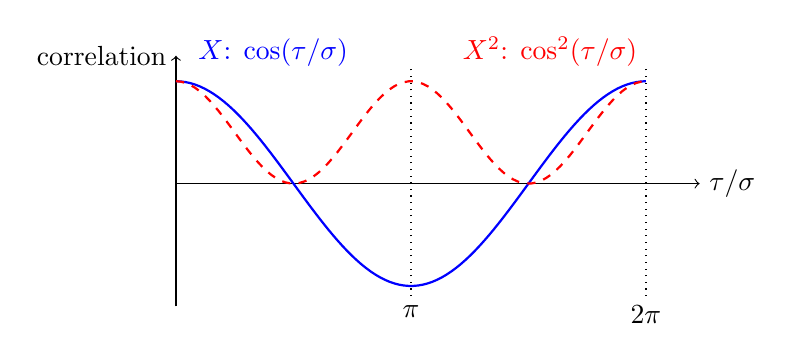
\begin{tikzpicture}[x=0.95cm,y=1.3cm]
 \draw[->] (0,-1.2)--(0,1.25) node[left] {correlation};
 \draw[->] (0,0)--(7,0) node[right] {$\tau/\sigma$};
 \draw[blue,thick,domain=0:6.283,samples=100] plot (\x,{cos(\x r)});
 \draw[red,dashed,thick,domain=0:6.283,samples=100] plot (\x,{cos(\x r)^2});
 \draw[dotted] (3.1416,-1.1)--(3.1416,1.12);
 \draw[dotted] (6.283,-1.1)--(6.283,1.12);
 \node[below] at (3.1416,-1.1) {$\pi$};
 \node[below] at (6.283,-1.1) {$2\pi$};
 \node[blue,above] at (1.3,1.05) {$X$: $\cos(\tau/\sigma)$};
 \node[red,above] at (5,1.05) {$X^2$: $\cos^2(\tau/\sigma)$};
\end{tikzpicture}
\caption{Exact Gaussian dynamics. The curves are analytic lag-one
correlations, not benchmark results. Half-period trajectories change the sign
of a draw but preserve its square; full-period trajectories preserve both.}
\label{fig:bf-modern-resonance}
\end{figure}

\subsection{Random lengths and NUTS}

If $P_\tau$ preserves $\pi$ for each fixed $\tau$, and $G$ is a
state-independent distribution over lengths, then
\begin{equation}
 \int\pi(dx)\int P_\tau(x,A)G(d\tau)
   =\int\pi(A)G(d\tau)=\pi(A).
 \label{eq:bf-modern-mixture-invariance}
\end{equation}
Thus randomizing length preserves invariance without a new correction,
provided each component kernel is valid and the distribution is fixed during
retained sampling. It spreads the risk of resonance. If
$\tau\sim\operatorname{Unif}(0,2\bar\tau)$ independently at every
Gaussian transition, direct integration yields
\begin{align}
 r_1&=\E[\cos(\tau/\sigma)]
       =\frac{\sin(2a)}{2a},\\
 r_2&=\E[\cos^2(\tau/\sigma)]
       =\frac12+\frac{\sin(4a)}{8a},
 \qquad a=\bar\tau/\sigma.
 \label{eq:bf-modern-random-length-correlations}
\end{align}
Here $X$ and $X^2-\sigma^2$ are eigenfunctions of the mixture with
eigenvalues $r_1$ and $r_2$. In particular, choosing $2\bar\tau=2\pi\sigma$
gives $r_1=0$ but $r_2=1/2$: the mean is decorrelated in one step while
variance estimation still has integrated autocorrelation time three.

NUTS uses the observed trajectory to decide how far to simulate
\citep[Section 3.1 and Algorithm 3]{hoffman2014nuts}. In Euclidean coordinates the familiar turning
conditions involve
$(x_+-x_-)^\top M^{-1}p_-$ and
$(x_+-x_-)^\top M^{-1}p_+$. Simply stopping when one becomes negative and
accepting the endpoint is not the NUTS algorithm: a state-dependent stopping
rule is not covered by \eqref{eq:bf-modern-mixture-invariance}. Tree building,
candidate selection and the exclusion of asymmetric subtrees provide the
required balance. That machinery removes a difficult manual length choice
but produces irregular work across chains. The extent of the resulting
accelerator cost depends on the implementation and target; it is not
determined by the name NUTS alone.

\subsection{ChEES and the stationary squared-jump identity}

For a square-integrable function $f$, define
\begin{equation}
 D_f=\tfrac12\E[(f(X')-f(X))^2].
 \label{eq:bf-modern-esjd-definition}
\end{equation}
At stationarity, $f(X)$ and $f(X')$ have equal means and variances, so
expansion of the square gives
\begin{equation}
 D_f=\Var_\pi(f)-\Cov(f(X),f(X'))
     =\Var_\pi(f)\{1-\rho_f(1)\}.
 \label{eq:bf-modern-esjd-identity}
\end{equation}
This connects a local movement objective to one-step correlation. It does
not determine every higher-lag correlation. In a reversible stationary chain,
a spectral representation makes the limitation precise. Normalize the
spectral measure $\mu_f$ to have total mass one. If the relevant sums are
integrable, then
\begin{equation}
 \rho_f(1)=\int\lambda\,\mu_f(d\lambda),\qquad
 \tau_{\rm int}(f)=\int\frac{1+\lambda}{1-\lambda}\,\mu_f(d\lambda).
 \label{eq:bf-modern-spectral-iat}
\end{equation}
The function $(1+\lambda)/(1-\lambda)$ is convex on $(-1,1)$ because
its second derivative is $4/(1-\lambda)^3$. Jensen's inequality therefore
implies
\begin{equation}
 \operatorname{ESS}_f
 =\frac{n}{\tau_{\rm int}(f)}
 \leq n\frac{1-\rho_f(1)}{1+\rho_f(1)}.
 \label{eq:bf-modern-esjd-bound}
\end{equation}
The right side is an upper bound, not a guarantee that maximizing a jump
criterion maximizes actual ESS \citep[Appendix B]{sountsov2022snaper}.

ChEES uses the centered squared radius
\begin{equation}
 f_{\rm ChEES}(x)=\tfrac12\|x-\mu\|^2,\qquad
 \mu=\E_\pi[X].
 \label{eq:bf-modern-chees}
\end{equation}
With the convention in \eqref{eq:bf-modern-esjd-definition}, the original
paper's ChEES criterion is $2D_{f_{\rm ChEES}}$; this constant factor does
not change its maximizer. The center is estimated during adaptation.
For independent Gaussian
coordinates with variances $\sigma_i^2$, the calculation above gives
\begin{equation}
 D_{f_{\rm ChEES}}(\tau)
       =\tfrac12\sum_i\sigma_i^4\sin^2(\tau/\sigma_i).
 \label{eq:bf-modern-chees-gaussian}
\end{equation}
To derive the coefficient, the variance of $X_i^2/2$ is
$\sigma_i^4/2$, its lag-one correlation is
$\cos^2(\tau/\sigma_i)$, and cross-coordinate terms vanish. Larger
variance directions receive weight $\sigma_i^4$, but sufficiently many
moderate directions can still outweigh one slow direction. Also, a large
jump obtained using a long trajectory may be poor value per gradient. These
motivate SNAPER \citep{hoffman2021chees,sountsov2022snaper}.

\subsection{SNAPER, endpoint derivatives and freezing}

Let $w$ be a unit principal direction estimated from the current ensemble.
SNAPER uses
\begin{equation}
 f_w(x)=\{w^\top(x-\mu)\}^2,\qquad
 C_w(\tau)=\frac{D_{f_w}(\tau)}{\tau}.
 \label{eq:bf-modern-snaper}
\end{equation}
Dividing by $\tau$ accounts for integration cost at fixed epsilon; optimizing
along $w$ focuses on a difficult direction rather than the sum of all
directions. Both changes remain proxies. The principal covariance direction
need not be the most difficult nonlinear or multimodal direction.

The pathwise derivative can be obtained without differentiating every
integration step. For an exact trajectory with initial state held fixed,
$d x_\tau/d\tau=M^{-1}p_\tau$. Holding $w$ and $\mu$ fixed while
differentiating,
\begin{align}
 \nabla f_w(x)&=2w\,w^\top(x-\mu),\\
 \frac{d}{d\tau}\frac{\{f_w(x_\tau)-f_w(x_0)\}^2}{2\tau}
 &=\frac{f_w(x_\tau)-f_w(x_0)}{\tau}
       \nabla f_w(x_\tau)^\top M^{-1}p_\tau
   -\frac{\{f_w(x_\tau)-f_w(x_0)\}^2}{2\tau^2}.
 \label{eq:bf-modern-snaper-derivative}
\end{align}
This is the quotient rule plus the endpoint velocity. It explains why a
trajectory objective need not require filter Hessians. A numerical algorithm
uses an annotated endpoint derivative and treats the rounded step count and
accept/reject behavior carefully; the exact derivative above is not an exact
derivative of a discontinuous rounded-and-rejected program
\citep[Appendix C]{sountsov2022snaper}. Such gradients propose adaptation
updates. They do not enter the acceptance ratio.

A principal direction can be estimated by stochastic power iteration. If
$z=x-\mu$, then $\E[zz^\top w]=\Cov(X)w$. An Oja-type update takes the
tangent component
\begin{equation}
 \widetilde w=w+\eta\{zz^\top w-w(w^\top z)^2\},\qquad
 w^+=\widetilde w/\|\widetilde w\|.
 \label{eq:bf-modern-oja}
\end{equation}
Its expectation moves toward covariance eigenvectors, subject to the usual
eigenvalue separation and stochastic-approximation conditions. An estimated
center, diagonal mass, length parameters and epsilon all change the
transition during adaptation. Their final values must be frozen before the
retained phase is interpreted using a fixed-kernel argument.

TensorFlow Probability 0.25.0 provides the kernel
\texttt{SNAPER\allowbreak Hamiltonian\allowbreak MonteCarlo}.
It adapts diagonal scaling,
the principal direction and trajectory length, but not epsilon; the
\texttt{sample\_snaper\_hmc} helper supplies dual averaging. The paper's
SGA implementation uses its own synthetic acceptance update, so the helper
should not be described as byte-for-byte reproduction of that tuning scheme.
The implementation requires at least two chains. Its concentrated-start
recommendation is an adaptation choice, not a justification for discarding
independent dispersed verification starts. Source availability reduces porting
effort; complete target, graph, GPU and checkpoint compatibility still needs
testing.

\section{Partial refreshment, MALT and MEADS}
\label{sec:bf-modern-persistence}

\subsection{The Ornstein--Uhlenbeck refreshment}

An underdamped Langevin process with mass $M$ and scalar friction $\gamma$
can be written
\begin{equation}
 dX_t=M^{-1}P_t\,dt,\qquad
 dP_t=-\nabla U(X_t)\,dt-\gamma P_t\,dt
          +\sqrt{2\gamma}M^{1/2}dW_t.
 \label{eq:bf-modern-langevin}
\end{equation}
During a refreshment substep with $X$ fixed, the linear stochastic equation
has solution
\begin{equation}
 P'=aP+\sqrt{1-a^2}M^{1/2}\xi,\qquad
 a=e^{-\gamma h},\quad\xi\sim\calN(0,I).
 \label{eq:bf-modern-ou}
\end{equation}
Indeed, multiply the momentum equation by $e^{\gamma t}$ and integrate.
The stochastic integral has covariance
$2\gamma M\int_0^h e^{-2\gamma(h-s)}ds=(1-e^{-2\gamma h})M$.
If $P\sim\calN(0,M)$, then $\Var(P')=a^2M+(1-a^2)M=M$. Moreover
$(P,P')$ is jointly Gaussian with equal marginal covariances and symmetric
cross-covariance $aM$, so its law is unchanged by exchange. The refreshment
kernel $Q$ therefore satisfies
\begin{equation}
 e^{-K(p)}Q(p,dp')=e^{-K(p')}Q(p',dp).
 \label{eq:bf-modern-ou-balance}
\end{equation}
The parameter $a$ trades momentum persistence against randomization. It does
not remove the need to choose a numerical step size.

\subsection{Why MALT sums deterministic energy errors}

MALT composes refreshment and leapfrog substeps in a symmetric Langevin
trajectory \citep[Sections 2--3]{rioudurand2023malt}. Consider the complete
realized path. Its probability ratio under time reversal contains the
endpoint density ratio $e^{-[H_{\rm end}-H_{\rm start}]}$, the Jacobians
of deterministic maps, and the ratios of refreshment probabilities. The
deterministic leapfrog Jacobians are one. From
\eqref{eq:bf-modern-ou-balance}, each refreshment contributes
\begin{equation}
 \frac{Q(p',dp)}{Q(p,dp')}=e^{K(p')-K(p)}.
 \label{eq:bf-modern-refresh-ratio}
\end{equation}
Decompose the total energy change into changes during deterministic
leapfrog substeps, $\Delta H_j^{\rm D}$, and refreshment changes
$\Delta K_j^{\rm O}$. The path log ratio becomes
\begin{equation}
 -\Delta H_{\rm total}+\sum_j\Delta K_j^{\rm O}
       =-\sum_j\Delta H_j^{\rm D}.
 \label{eq:bf-modern-malt-path-ratio}
\end{equation}
The OU terms cancel rather than being counted as numerical energy errors.
A reversal of the complete path, with the momentum sign convention and
palindromic refreshment schedule, provides the extended-space involution.
Accepting with $1\wedge\exp(-\sum_j\Delta H_j^{\rm D})$ is therefore
the relevant correction. Full momentum refresh at trajectory boundaries
allows the accepted position transition to be used without inheriting a
persistent rejected momentum.

For unit mass, the deterministic local error can be expressed using positions
alone. Let $y=x+h v_{1/2}$, and write $g_x=\nabla U(x)$,
$g_y=\nabla U(y)$. The endpoint velocities of the leapfrog substep are
\begin{equation}
 v_0=(y-x)/h+(h/2)g_x,\qquad
 v_1=(y-x)/h-(h/2)g_y.
 \label{eq:bf-modern-malt-velocities}
\end{equation}
Expanding the squared norms gives
\begin{align}
 E_h(x,y)&=U(y)-U(x)+\tfrac12(\|v_1\|^2-\|v_0\|^2)\\
 &=U(y)-U(x)-\tfrac12(y-x)^\top(g_y+g_x)
              +\tfrac{h^2}{8}(\|g_y\|^2-\|g_x\|^2).
 \label{eq:bf-modern-malt-local-error}
\end{align}
This reproduces the paper's local error, equation (5). Summing it along the
path yields the acceptance exponent. Using only the total endpoint
Hamiltonian difference, including refreshment randomness, computes a
different ratio.

Adaptive MALT estimates scaling, damping, epsilon and trajectory length
\citep{rioudurand2023adaptive}. Its empirical results distinguish efficiency
per iteration from efficiency per gradient. It is sometimes slightly less
gradient-efficient than uniformly randomized HMC using SNAPER adaptation,
despite competitive iteration efficiency. The author implementation in
TensorFlow Probability's discussion directory uses JAX/FunMC; its location
does not make it an installed TensorFlow transition kernel.

\subsection{Generalized HMC and ensemble adaptation}

Generalized HMC retains part of its momentum between transitions. One valid
construction composes OU refreshment with the involutive leapfrog proposal
$R\Phi$, accepts or rejects against $H$, and then applies an unconditional
momentum flip $R$. The final flip preserves the joint target. In this
equivalent convention, an accepted move ends with the forward momentum,
whereas a rejected move flips it. Repeated rejections can therefore undo
directional progress; correct momentum handling is part of the algorithm,
not a cosmetic implementation detail.

MEADS adds ensemble-based scale adaptation and a persistent slice construction
\citep{hoffman2022meads}. A slice variable has joint unnormalized density
\begin{equation}
 \rho(x,p,s)=\mathbf1\{0<s<e^{-H(x,p)}\}.
 \label{eq:bf-modern-slice-joint}
\end{equation}
Integrating over $s$ gives $e^{-H(x,p)}$. A volume-preserving reversible
proposal at fixed $s$ can move only within the slice; a valid update of $s$
must preserve this joint measure. Reusing an arbitrary uniform variate across
ordinary MH tests is not sufficient. The paper supplies a particular
persistent-slice transition, together with ensemble estimates that avoid
direct Hessian evaluation.

The conditional-independence argument behind folded ensemble adaptation can
be stated precisely. Partition chains into a block $A$ and its complement.
Choose parameters $\lambda=\Lambda(X_{-A})$ only from the complementary
block. Conditional on $X_{-A}$, suppose the transition $P_\lambda$ for $A$
preserves $\pi^{\otimes |A|}$. Then
\begin{align}
 &\int\pi^{\otimes |A|}(dx_A)\,\pi^{\otimes|A^c|}(dx_{-A})
                P_{\Lambda(x_{-A})}(x_A,dx_A')\\
 &\hspace{2cm}=\pi^{\otimes |A|}(dx_A')\,\pi^{\otimes|A^c|}(dx_{-A}).
 \label{eq:bf-modern-folded-invariance}
\end{align}
The product target is preserved. Sequentially changing the held-out block
preserves it as well. If the parameter estimate uses the very state being
updated, the displayed conditional argument no longer applies. MEADS's
fold construction must therefore be preserved when claiming its exact
ensemble-adaptation property. For a first local implementation, finite
adaptation followed by a completely frozen kernel is simpler to validate.

\section{Microcanonical dynamics and the MAMS correction}
\label{sec:bf-modern-mams}

\subsection{A velocity of fixed norm}

MAMS uses a direction $u$ on the unit sphere $S^{d-1}$ instead of a Gaussian
momentum \citep{robnik2025mams}. For $d>1$, define
\begin{equation}
 \dot x=u,\qquad
 \dot u=-\frac{1}{d-1}(I-uu^\top)g(x),\qquad
 g(x)=\nabla U(x).
 \label{eq:bf-modern-microcanonical-dynamics}
\end{equation}
The projected force changes direction while preserving speed. Indeed,
\begin{equation}
 \frac{d}{dt}\|u\|^2
 =-\frac{2}{d-1}\{u^\top g-\|u\|^2u^\top g\}=0
 \quad\hbox{when }\|u\|=1.
 \label{eq:bf-modern-sphere-norm}
\end{equation}
The factor $d-1$ is the dimension of the tangent space. It makes this formula
undefined at $d=1$; a one-dimensional specialization requires a different
construction, not an arbitrary division guard.

The name microcanonical can obscure an important distinction: these equations
are not ordinary canonical Hamiltonian equations in $(x,u)$ with Gaussian
kinetic energy. They are a time-rescaled, fixed-speed construction with
stationary measure
\begin{equation}
 \rho(x,u)\,dx\,d\omega(u)
       =\pi(x)\,dx\,\frac{d\omega(u)}{|S^{d-1}|},
 \label{eq:bf-modern-sphere-target}
\end{equation}
where $d\omega$ is sphere surface measure. The measure, and not merely the
dimension of an array storing $u$, determines the Jacobian in the acceptance
calculation.

\subsection{Derivation of the stationary measure}

For fixed $a\in\R^d$, the tangent field
$v(u)=(I-uu^\top)a$ has intrinsic divergence
\begin{equation}
 \operatorname{div}_{S^{d-1}}v=-(d-1)u^\top a.
 \label{eq:bf-modern-sphere-divergence}
\end{equation}
To see this without a coordinate chart, let $P=I-uu^\top$ and use an
orthonormal tangent frame. The ambient derivative is
$Dv=-u a^\top-(u^\top a)I$. Taking the tangent trace gives
$\tr(P Dv P)=-(u^\top a)\tr(P)=-(d-1)u^\top a$, since $Pu=0$.
With $a=-g/(d-1)$, the velocity field in
\eqref{eq:bf-modern-microcanonical-dynamics} therefore has divergence
$u^\top g$. Its position component has zero position divergence. The
stationary continuity equation is satisfied because
\begin{align}
 \operatorname{div}(\rho b)
 &=\rho\{\operatorname{div}b+b\cdot\nabla\log\rho\}\\
 &=\rho\{u^\top g-u^\top g\}=0.
 \label{eq:bf-modern-sphere-stationarity}
\end{align}
This derivation assumes sufficient smoothness and a nonexplosive flow for the
continuity argument. It establishes the invariant density of the exact
dynamics. It does not prove ergodicity of the deterministic motion or remove
finite-step integration bias \citep[Appendix B.4]{robnik2025mams}.

The comparison with canonical HMC is useful. In canonical coordinates the
flow preserves volume and density separately through energy conservation.
Here density changes along the position trajectory and volume changes in the
sphere directions compensate. The numerical method must keep track of that
compensation.

\subsection{The exact force subflow}

Split the dynamics into a drift $A_h:(x,u)\mapsto(x+hu,u)$ and a force
subflow $B_h$ holding $x$ fixed. For nonzero $g$, put
\begin{equation}
 e=-g/\|g\|,\qquad k=\|g\|/(d-1),\qquad
 c_0=e^\top u_0,\qquad \delta=kh.
 \label{eq:bf-modern-force-definitions}
\end{equation}
Then $\dot u=k(e-(e^\top u)u)$. The scalar projection $c=e^\top u$
satisfies $\dot c=k(1-c^2)$. Integrating
$dc/(1-c^2)=k\,dt$ gives
\begin{equation}
 c_h=\frac{\sinh\delta+c_0\cosh\delta}
            {\cosh\delta+c_0\sinh\delta}.
 \label{eq:bf-modern-force-projection}
\end{equation}
For $|c_0|<1$ this follows from the addition formula for $\tanh$; the formula
also has well-defined limits at $c_0=\pm1$. Write $r=u-ce$, with $e^\top r=0$.
The transverse equation is $\dot r=-kc r$. Define
$D_h=\cosh\delta+c_0\sinh\delta$. Since
$d\log D_t/dt=kc_t$, integration yields $r_h=r_0/D_h$. Combining the
parallel and perpendicular components gives the closed form
\begin{equation}
 B_h(u_0)=
 \frac{u_0+e\{\sinh\delta+(\cosh\delta-1)c_0\}}
      {D_h}.
 \label{eq:bf-modern-force-map}
\end{equation}
The denominator is positive for finite $\delta$ and $c_0\in[-1,1]$, since
$\cosh\delta>|\sinh\delta|$. A direct norm check uses
\begin{equation}
 1-c_0^2+(\sinh\delta+c_0\cosh\delta)^2
       =(\cosh\delta+c_0\sinh\delta)^2=D_h^2.
 \label{eq:bf-modern-force-norm-identity}
\end{equation}
Thus the update remains on the sphere. At $g=0$, the correct limiting update
is $B_h(u)=u$; constructing $e$ by dividing by zero is unnecessary.

\subsection{The surface Jacobian and accumulated work}

During $B_h$, the sphere divergence is
$u^\top g=-(d-1)kc$. Liouville's formula on the sphere and the expression
for $D_h$ imply
\begin{align}
 \log J_{B_h}(u_0)
 &=\int_0^h\operatorname{div}_{S^{d-1}}\dot u_t\,dt\\
 &=-(d-1)\int_0^h kc_t\,dt
   =-(d-1)\log D_h.
 \label{eq:bf-modern-force-jacobian}
\end{align}
This is the negative of the paper's quantity
$\Delta K=(d-1)\log D_h$ \citep[equation (8)]{robnik2025mams}. Here
$\Delta K$ denotes a volume correction; it is not a change in
$\|u\|^2/2$, which is constant.

A symmetric composition such as $B_{h/2}A_hB_{h/2}$ is reversible under
$R(x,u)=(x,-u)$. The drift is volume preserving, while force substeps
contribute \eqref{eq:bf-modern-force-jacobian}. Proposition
\ref{prop:bf-modern-involution} therefore yields
\begin{align}
 \log r&=-U(x')+U(x)+\sum_j\log J_{B_j},\\
 W&=U(x')-U(x)+(d-1)\sum_j\log D_j,\\
 a&=\min\{1,e^{-W}\}.
 \label{eq:bf-modern-mams-acceptance}
\end{align}
Potential changes telescope across drift substeps. The signs matter:
subtracting rather than adding $\Delta K$ in $W$ would produce the wrong
accepted measure. The inspected BlackJAX implementation accumulates this
integrator work and adds the endpoint log-density difference with precisely
this sign.

For numerical stability, the equivalent identity
\begin{equation}
 D_h=\tfrac12\{(1+c_0)e^\delta+(1-c_0)e^{-\delta}\}
 \label{eq:bf-modern-stable-force-denominator}
\end{equation}
permits a log-sum-exp calculation of $\log D_h$, including limiting zero
weights when $c_0=\pm1$. The vector update needs a correspondingly stable
implementation for large $|\delta|$. A guard that merely clips $\delta$
changes the map and its Jacobian; it cannot silently retain the original
correction. Reversibility, surface Jacobian and zero-gradient limits should
be tested together.

\subsection{Sphere refreshment and the stochastic variant}

A full refresh is $u=\xi/\|\xi\|$ for
$\xi\sim\calN(0,I)$; rotational invariance gives the uniform sphere law.
A partial refresh used in microcanonical implementations has the form
\citep{robnik2025mclmc,robnik2025mams}
\begin{equation}
 u'=\frac{u+\eta\xi}{\|u+\eta\xi\|},\qquad \eta>0.
 \label{eq:bf-modern-sphere-refresh}
\end{equation}
At a fixed state-independent $\eta$, its transition density with respect to
surface measure is
\begin{equation}
 q(u'\mid u)=(2\pi\eta^2)^{-d/2}\int_0^\infty r^{d-1}
    \exp\!\left[-\frac{r^2+1-2r u^\top u'}{2\eta^2}\right]dr.
 \label{eq:bf-modern-sphere-refresh-density}
\end{equation}
This follows by writing a Gaussian draw in polar coordinates. The expression
depends only on $u^\top u'$, so $q(u'\mid u)=q(u\mid u')$ and the uniform
sphere law is reversible. The zero-noise limit is the identity transition.
In a symmetric stochastic path, these refreshment ratios cancel; the
deterministic subflow Jacobians still accumulate. The extended-path argument
in MAMS's Appendix A handles the actual noise and rejection conventions.
State-dependent refreshment strengths would require rechecking the ratio.

MAMS consequently has several controls: a geometry or preconditioner,
epsilon, a trajectory length and, in its Langevin variant, a decoherence
scale. The paper uses automatic adaptation, including a preliminary
preconditioner estimate---in practice from NUTS---and length selection using
autocorrelation information. Its practical acceptance target is 0.90, with
0.99 used for its funnel experiment; these are author settings, not universal
optimal values. The paper calls physical trajectory length $L$. This chapter
uses $\tau$ for physical length and $L$ for an integer integration count,
with $\tau\approx L\epsilon$, to avoid confusion with BayesFilter's tuning
interface.

\section{Unadjusted bias and the LAPS warm-up strategy}
\label{sec:bf-modern-laps}

\subsection{What a finite-step unadjusted chain samples}

An exact invariant diffusion or deterministic flow does not imply that its
finite-step discretization has the same invariant distribution. A Gaussian
calculation exposes the distinction without asymptotic notation. Use the
unit-mass leapfrog in \eqref{eq:bf-modern-leapfrog} for
$U(x)=x^2/(2\sigma^2)$, refresh momentum independently before each single
step, and omit MH. With $h=\epsilon$ and $y=h^2/\sigma^2$, its matrix is
\begin{equation}
 \begin{pmatrix}x'\\p'\end{pmatrix}
 =
 \begin{pmatrix}
  1-y/2 & h\\
  -h\sigma^{-2}(1-y/4)&1-y/2
 \end{pmatrix}
 \begin{pmatrix}x\\p\end{pmatrix}.
 \label{eq:bf-modern-gaussian-leapfrog-matrix}
\end{equation}
For $0<y<4$ the position recursion has coefficient $a=1-y/2$ with
$|a|<1$. If its stationary variance is $v_h$, then
$v_h=a^2v_h+h^2$. Solving gives
\begin{equation}
 v_h=\frac{h^2}{1-a^2}
     =\frac{\sigma^2}{1-y/4},\qquad
 b=\frac{v_h}{\sigma^2}-1=\frac{y/4}{1-y/4}.
 \label{eq:bf-modern-gaussian-biased-variance}
\end{equation}
Every positive stable step size inflates the variance in this scheme.
Increasing the number of iterations only estimates $v_h$ more accurately;
it does not make $v_h$ equal to $\sigma^2$. Different splitting conventions
can have different bias, so their formulas must not be exchanged silently.

The energy error contains useful information about this bias. Let $A$ be the
matrix in \eqref{eq:bf-modern-gaussian-leapfrog-matrix},
$D=\diag(\sigma^{-2},1)$ and $S=\diag(v_h,1)$. At the stationary
unadjusted input, $z=(x,p)\sim\calN(0,S)$, and
\begin{equation}
 \Delta H=\tfrac12 z^\top Qz,\qquad Q=A^\top D A-D.
 \label{eq:bf-modern-gaussian-error-quadratic}
\end{equation}
For a centered Gaussian vector, expansion using fourth moments gives
$\Var(z^\top Qz)=2\tr(QSQS)$. Hence
\begin{align}
 \Var(\Delta H)&=\tfrac12\tr(QSQS)
          =\frac{y^3}{16(1-y/4)}\\
 &=\frac{4b^3}{(1+b)^2}
   =F(b^2),\qquad F(D)=\frac{4D^{3/2}}{(1+\sqrt D)^2}.
 \label{eq:bf-modern-gaussian-eevpd}
\end{align}
For an explicit check, substitution into $Q$ gives
\begin{equation}
 Q_{11}=-\frac{y^2(1-y/4)}{4\sigma^2},\qquad
 Q_{12}=Q_{21}=\frac{hy(1-y/2)}{4\sigma^2},\qquad
 Q_{22}=\frac{y^2}{4}.
 \label{eq:bf-modern-gaussian-error-entries}
\end{equation}
Consequently $Q_{11}v_h=-y^2/4$ and
$\tfrac12\tr(QSQS)=y^4/16+
y^3(1-y/2)^2/[16(1-y/4)]$. Combining the numerator uses
$y(1-y/4)+(1-y/2)^2=1$ and yields
\eqref{eq:bf-modern-gaussian-eevpd}. This is a relation between the
stationary error of this specified integrator and a specified covariance
bias, not a relation between arbitrary transient error and arbitrary
observables.

For independent Gaussian eigendirections, independent energy errors add.
With $b_i=v_{h,i}/\sigma_i^2-1$, define
\begin{equation}
 D_{\rm cov}=\frac1d\sum_i b_i^2,\qquad
 E=\frac1d\Var(\Delta H)=\frac1d\sum_i F(b_i^2).
 \label{eq:bf-modern-eevpd-multivariate}
\end{equation}
In the isotropic case $E=F(D_{\rm cov})$ exactly. More generally,
\begin{align}
 F'(D)&=\frac{2\sqrt D(3+\sqrt D)}{(1+\sqrt D)^3}>0,\\
 F''(D)&=\frac{3-4\sqrt D-D}{\sqrt D(1+\sqrt D)^4}.
 \label{eq:bf-modern-bias-function-derivatives}
\end{align}
The numerator of the second derivative is positive for
$0<D<11-4\sqrt7$. If every $b_i^2$ lies in that interval, Jensen's
inequality gives $F(D_{\rm cov})\leq E$, and monotonicity implies
$D_{\rm cov}\leq F^{-1}(E)$. This is a sufficient restricted Gaussian
bound. The broader statement and its admissible range in
\citet[Theorem 4.2 and Appendix B]{robnik2026unadjusted} require their
stated conditions. Neither argument proves a universal microcanonical or
non-Gaussian error bound.

For small $h$, $b=O(h^2)$, $D_{\rm cov}=O(h^4)$ and
$E=O(h^6)$. Thus a sixth-root adjustment
$h_{\rm new}=h(E_{\rm wanted}/E)^{1/6}$ has a local scaling rationale.
Outside that regime, the relation need not be accurate. The cited paper's
non-Gaussian experiments include a Brownian-motion case where the proposed
bound underpredicts observed bias by about a factor of 1.5. Its June 2026
revision provides useful evidence for adaptation, not a general certificate
of approximation error.

\subsection{The ideal bias--contraction schedule}

LAPS uses an unadjusted microcanonical transient, followed by adjusted MAMS
\citep{robnik2026laps}. Its theoretical motivation can be reconstructed from
two assumptions. Let $D$ now denote a genuine distance satisfying the
triangle inequality. Assume $K_h$ has invariant distribution $\pi_h$, with
\begin{align}
 D(\pi_h,\pi)&\leq C_{\rm b}h^\kappa,\\
 D(\rho K_h,\pi_h)&\leq(1-c)D(\rho,\pi_h),\qquad 0<c<1,
 \label{eq:bf-modern-laps-assumptions}
\end{align}
where the constants are uniform over the step sizes being used. Two triangle
inequalities imply
\begin{align}
 D(\rho K_h,\pi)
 &\leq D(\rho K_h,\pi_h)+D(\pi_h,\pi)\\
 &\leq(1-c)D(\rho,\pi)+(2-c)C_{\rm b}h^\kappa.
 \label{eq:bf-modern-laps-contraction}
\end{align}
This separates contraction of initialization error from the numerical bias
floor. Suppose one transition simulates fixed physical length $\tau$ and
therefore costs approximately $\tau/h$ gradient evaluations. If
$D_t=D(\rho_t,\pi)$, the lower bound on improvement per gradient is
\begin{equation}
 R(h)=\frac h\tau\{cD_t-(2-c)C_{\rm b}h^\kappa\}.
 \label{eq:bf-modern-laps-rate}
\end{equation}
Differentiating gives
$\tau R'(h)=cD_t-(\kappa+1)(2-c)C_{\rm b}h^\kappa$.
The positive maximizer consequently satisfies
\begin{equation}
 C_{\rm b}h_t^\kappa
   =\frac{cD_t}{(2-c)(\kappa+1)},\qquad
 D_{t+1}\leq\left(1-\frac{c\kappa}{\kappa+1}\right)D_t.
 \label{eq:bf-modern-laps-ideal-schedule}
\end{equation}
This reproduces the argument in LAPS Appendix A. The optimum is of the
specified lower bound under uniform contraction and cost assumptions. It is
not a universal optimum for arbitrary MCMC. In particular, the moment
statistic used in practice below is not a general distance with the triangle
inequality, so it cannot simply be substituted into this proof.

\subsection{Equipartition as a measurable but incomplete diagnostic}

The target moments needed to measure $D_t$ are generally unknown. LAPS uses
an integration-by-parts identity. Let $\rho$ describe the current ensemble,
with mean $m_\rho$. Define
\begin{equation}
 V_{ij}(\pi,\rho)
 =\E_\rho[-(X_i-m_{\rho,i})\partial_j\log\pi(X)],\qquad
 \widetilde D=\frac1d\|I-V\|_F^2.
 \label{eq:bf-modern-equipartition}
\end{equation}
Assume the relevant expectations exist, $\pi$ is differentiable and the
boundary term $(x_i-m_{\pi,i})\pi(x)$ vanishes in the integration-by-parts
calculation. At the target,
\begin{align}
 V_{ij}(\pi,\pi)
 &=-\int(x_i-m_{\pi,i})\partial_j\pi(x)\,dx\\
 &=-\left[\hbox{boundary term}\right]
      +\int\partial_j(x_i-m_{\pi,i})\pi(x)\,dx
   =\delta_{ij}.
 \label{eq:bf-modern-equipartition-proof}
\end{align}
The identity uses the score of the actual density, including coordinate
Jacobians. A generic force $b$ cannot be inserted without a new argument.
Bounded domains and heavy tails require particular care with the boundary
term and existence of moments.

The implication $\rho=\pi\Rightarrow V=I$ does not have a general converse.
For $\pi=\calN(0,I)$, $-\nabla\log\pi(x)=x$. If
$\rho=\calN(m,S)$, then
\begin{equation}
 V=\E_\rho[(X-m)X^\top]=S.
 \label{eq:bf-modern-equipartition-gaussian}
\end{equation}
Thus $S=I$ makes the diagnostic zero for every mean $m$, however far it is
from the target. The full matrix detects a wrong covariance, but its
diagonal reduction
\begin{equation}
 \widetilde D_{\rm diag}=\frac1d\sum_i(1-V_{ii})^2
 \label{eq:bf-modern-equipartition-diagonal}
\end{equation}
does not. For instance, $S=\left(\begin{smallmatrix}1&r\\r&1\end{smallmatrix}\right)$
with $0<|r|<1$ has zero diagonal diagnostic and wrong correlation. Even the
full matrix cannot distinguish all non-Gaussian distributions: a centered
smooth mixture
$\tfrac12\calN(-a,1-a^2)+\tfrac12\calN(a,1-a^2)$, $0<a<1$, has variance
one and therefore $V=1$, while its fourth moment
$3-2a^4$ differs from the standard Gaussian value three. These are exact
counterexamples, not merely concerns about finite ensemble size.

The LAPS paper explicitly calls $\widetilde D$ a proxy and proves separation
only on a restricted zero-mean Gaussian family. The examples above explain
why one needs additional means, dependence, tail and mode diagnostics when
using it for adaptation. Empirical moment fluctuations can also stabilize
inside a single missed mode. A stable statistic is informative about that
statistic, not all posterior quantities.

\subsection{From the proxy to an operational schedule}

In the paper's scheme, select a fraction $0<C<1$ and set
\begin{equation}
 D_{\rm wanted}=C\widetilde D_t,\qquad
 E_{\rm wanted}=F(D_{\rm wanted}),\qquad
 h_{t+1}=h_t\left(\frac{E_{\rm wanted}}{\widehat E_t}\right)^{1/6}.
 \label{eq:bf-modern-laps-practical-schedule}
\end{equation}
The first assignment expresses a desired numerical bias below the estimated
current error; the second borrows the Gaussian relationship; the third uses
the small-step energy-error scaling. Each link has assumptions. In
particular, $\widehat E_t$ is measured during a transient, whereas
\eqref{eq:bf-modern-gaussian-eevpd} was derived at an unadjusted stationary
law. Finite ensembles, small denominators, heavy tails and a wrong proxy can
all mislead the update. A bounded implementation must handle them explicitly
and report why adaptation ended.

After the unadjusted stage, LAPS applies a diagonal reparameterization, turns
on MH and adapts the final adjusted settings. The paper uses a practical
stopping rule based on fluctuations of second moments, not a proof that all
initialization bias has disappeared. For posterior reporting, discard every
unadjusted and adaptive draw, freeze all shared settings and assess the final
fixed kernel. If chains shared adaptation, freezing stops further coupling
but does not instantly make their current states independent or stationary.

The inspected BlackJAX revision contains choices different from the paper.
Its desired error is coded as $C\,\mathrm{bias}^{3/8}$, with the paper's
$F(C\widetilde D)$ expression commented out. Its diagonal statistic uses
$-x_i\partial_i\log\pi(x)$ without centering, and its fluctuation function
uses variance divided by squared mean rather than relative standard
deviation. The centered mean-shift counterexample therefore does not apply
unchanged to that uncentered code, but neither statistic determines a general
distribution. The adjusted epsilon freezes through an acceptance-tolerance
flag; the first tolerance-satisfying update can still change epsilon before
the next call freezes it. A faithful local port must resolve these definitions
and test the setting actually frozen. These observations concern the pinned
current source, not an identified source revision of the published benchmark.

\subsection{Gradient work and parallel latency}

Table~\ref{tab:bf-modern-mams-benchmarks} reports selected entries from the
MAMS paper. The criterion is a normalized squared error in the worst second
moment below 0.01, taking median error across at least 128 chains. Tuning work
is excluded. A small ratio in one model does not invalidate the method, but
it does limit a blanket several-fold claim.
\begin{table}[htbp]
\centering\small
\begin{tabular}{lrrr}
\toprule
Author target & NUTS gradients & MAMS gradients & Ratio\\
\midrule
Gaussian & 19,652 & 3,249 & 6.05\\
Banana & 95,519 & 14,078 & 6.78\\
Bimodal & 210,758 & 139,418 & 1.51\\
Brownian & 29,816 & 13,528 & 2.20\\
Stochastic volatility & 843,768 & 430,088 & 1.96\\
\bottomrule
\end{tabular}
\caption{Selected MAMS Table 1 entries \citep{robnik2025mams}. Ratios are
descriptive arithmetic on the authors' reported counts, not local timings
or uncertainty-qualified rankings for the present consumers.}
\label{tab:bf-modern-mams-benchmarks}
\end{table}

LAPS's experiments use an NVIDIA A100 with 40 GB. Its Table 1 uses 4,096
chains; Table 2 uses 256. For stochastic volatility, Table 2 reports 29,900
gradients for sequential NUTS, 1,100 per LAPS chain and 281,600 across the
LAPS ensemble \citep{robnik2026laps}. The last two figures satisfy
$256\times1{,}100=281{,}600$. Under the idealized model of perfectly
synchronized work, its latency ratio to that sequential comparator is
\begin{equation}
 \frac{C_{\rm LAPS}}{C_{\rm NUTS}}
 \approx\frac{1{,}100\,c_{\nabla}(256)}
              {29{,}900\,c_{\nabla}(1)}.
 \label{eq:bf-modern-laps-work-latency}
\end{equation}
Per-chain work is about 27 times smaller, but total gradient work is about
9.4 times larger. The idealized latency gain requires
$c_{\nabla}(256)/c_{\nabla}(1)<29{,}900/1{,}100$ before other overheads.
This calculation is not a fair complete local benchmark by itself: a local
NUTS baseline may also be batched, compilation and adaptation must be counted,
and a requested MCSE may require more than one final draw per chain.
The paper provides motivation to measure batch scaling, not permission to
assume it for Kalman, UKF or QZ calculations.

\section{Geometry and initialization}
\label{sec:bf-modern-geometry}

\subsection{Affine whitening and nonlinear funnels}

For a Gaussian target, let $\Sigma=AA^\top\in\R^{d\times d}$ be its symmetric
positive-definite covariance, with $A$ invertible. The map $x=\mu+Az$
gives a standard normal density for $z$. Substitution into
\eqref{eq:bf-modern-transformed-target} gives
\begin{equation}
 -\tfrac12(x-\mu)^\top\Sigma^{-1}(x-\mu)
       +\log|\det A|= -\tfrac12z^\top z+\hbox{constant}.
 \label{eq:bf-modern-affine-whitening}
\end{equation}
For ordinary Gaussian HMC in the original coordinates, equal oscillation
frequencies correspond to $M=\Sigma^{-1}$ in the convention
$K(p)=p^\top M^{-1}p/2$. Libraries sometimes expose $M^{-1}$ as their
\emph{inverse mass} parameter, so verbal descriptions of mass adaptation are
ambiguous unless this convention is stated. Whitening and mass adaptation
repair constant linear anisotropy. They cannot generally remove
position-dependent conditional scales.

Consider the funnel
\begin{equation}
 V\sim\calN(0,s^2),\qquad X_i\mid V=v\sim\calN(0,e^v),
       \quad i=1,\ldots,m.
 \label{eq:bf-modern-funnel}
\end{equation}
Its log density, up to a constant, is
\begin{equation}
 -\frac{v^2}{2s^2}-\frac m2v-\frac12e^{-v}\sum_i x_i^2.
 \label{eq:bf-modern-funnel-centered}
\end{equation}
The child-coordinate curvature is $e^{-v}$ and becomes arbitrarily large in
the neck. Let $v=sz_0$ and $x_i=e^{v/2}z_i$. The Jacobian is block
triangular, with determinant $s e^{mv/2}$. Adding its logarithm cancels the
linear $-mv/2$ term and yields
\begin{equation}
 \log\pi_z(z)=-\tfrac12z_0^2-\tfrac12\sum_i z_i^2+\hbox{constant}.
 \label{eq:bf-modern-funnel-whitened}
\end{equation}
Thus exact noncentering solves this analytic geometry problem. It does not
show that an affine tuning procedure ought to solve the centered funnel.

A partial-whitening example is equally useful. Use
$x_i=e^{v/2-\delta(v)}z_i$ and retain $v$ as a coordinate. Its transformed
log density is
\begin{equation}
 \log\pi(v,z)=-\frac{v^2}{2s^2}-m\delta(v)
                    -\frac12e^{-2\delta(v)}\sum_i z_i^2+\hbox{constant}.
 \label{eq:bf-modern-funnel-partial}
\end{equation}
The child Hessian of the negative log density is
$e^{-2\delta(v)}I$. If $|\delta(v)|\leq a$, its eigenvalues are bounded
between $e^{-2a}$ and $e^{2a}$. This bounds that block only: derivatives of
$\delta$ create cross terms and curvature in $v$. It is wrong to infer a
global full-Hessian bound from this child-coordinate bound. Exact and
residual-map fixtures distinguish map correctness from robustness to remaining
geometry.

\subsection{What neural transport learns}

For base density $\phi(z)$ and invertible $F_\lambda$, the induced density
$q_\lambda$ obeys
$\log q_\lambda(F_\lambda(z))=\log\phi(z)-\log|\det J_{F_\lambda}(z)|$.
The reverse-KL objective is therefore
\begin{align}
 \mathrm{KL}(q_\lambda\|\pi)
 &=\E_{Z\sim\phi}\big[
      \log\phi(Z)-\log|\det J_{F_\lambda}(Z)|
                     +U(F_\lambda(Z))\big]+\log Z_\pi.
 \label{eq:bf-modern-neutra-objective}
\end{align}
The unknown constant $Z_\pi=\int e^{-U(x)}dx$ does not affect optimization.
This is a training objective for useful coordinates, not a posterior-error
certificate \citep{hoffman2019neutra}. Undercoverage of a mode contributes
little when that mode is rarely sampled by $q_\lambda$. The final transformed
target must still use \eqref{eq:bf-modern-transformed-target}, not the learned
approximation alone.

Once frozen, the same map can be used by ordinary HMC, SNAPER or MAMS.
Consequently a fair kernel comparison holds the map fixed. An end-to-end
comparison may let each method construct geometry, but must then count fitting,
inverse-map evaluation for matched model starts, forward/log-Jacobian work
and transformed gradients. The current BayesFilter architecture policy selects
configured Huang DSF/NAF for the October 2026 forward/reverse training study,
and the repaired author IAF outside that study. Architecture selection and
successful training are separate from map validity, tail coverage and
downstream sampling accuracy.

\subsection{Pathfinder from a quadratic expansion}

Pathfinder constructs Gaussian approximations along optimization paths
\citep{zhang2022pathfinder}. Let
$x_k$ be an L-BFGS iterate minimizing $U$, $g_k=\nabla U(x_k)$, and $B_k$
a positive-definite inverse-Hessian approximation. A local quadratic model is
\begin{equation}
 U(x)\approx U(x_k)+g_k^\top(x-x_k)
               +\tfrac12(x-x_k)^\top B_k^{-1}(x-x_k).
 \label{eq:bf-modern-pathfinder-quadratic}
\end{equation}
Completing the square gives mean and covariance
\begin{equation}
 \mu_k=x_k-B_k g_k,\qquad q_k=\calN(\mu_k,B_k).
 \label{eq:bf-modern-pathfinder-gaussian}
\end{equation}
In particular, the Gaussian is centered at the stationary point of the local
quadratic, not necessarily the current iterate. If $s_k=x_{k+1}-x_k$ and
$y_k=g_{k+1}-g_k$, the full BFGS inverse update is
\begin{equation}
 B_{k+1}=(I-\rho_k s_k y_k^\top)B_k(I-\rho_k y_k s_k^\top)
                  +\rho_k s_k s_k^\top,\qquad
 \rho_k=(y_k^\top s_k)^{-1}.
 \label{eq:bf-modern-bfgs}
\end{equation}
Multiplying by $y_k$ verifies the secant equation $B_{k+1}y_k=s_k$.
If $y_k^\top s_k>0$ and $B_k$ is positive definite, the quadratic form of
the update is the sum of a nonnegative transformed $B_k$ form and
$\rho_k(s_k^\top v)^2$; their simultaneous vanishing forces $v=0$.
This proves positive definiteness. Limited-memory representations retain
selected $(s,y)$ pairs and exploit a diagonal-plus-low-rank form instead of
storing a dense $d\times d$ matrix. Negative or negligible curvature must be
handled explicitly, not treated as a valid Gaussian covariance.

For each proposed $q_k$, the evidence lower bound satisfies
\begin{equation}
 \mathcal L(q_k)=\E_{q_k}[\log\widetilde\pi(X)-\log q_k(X)]
        =\log Z_\pi-\mathrm{KL}(q_k\|\pi).
 \label{eq:bf-modern-pathfinder-elbo}
\end{equation}
Maximizing an estimate of $\mathcal L$ along the path chooses a promising
approximation; the estimated maximum has Monte Carlo selection uncertainty.
The inspected Stan implementation checks curvature and stores the
approximation with favorable estimated ELBO. A good local approximation can
provide initial states and scaling, but missing modes remain possible.

The paper's multipath importance step is best understood on an augmented
space. If $J$ paths supply densities $q_j$, define
\begin{equation}
 q(x,j)=J^{-1}q_j(x),\qquad \pi(x,j)=J^{-1}\pi(x).
 \label{eq:bf-modern-pathfinder-augmented}
\end{equation}
The importance ratio is $\widetilde\pi(x)/q_j(x)$ for a draw from path $j$;
the factors $J^{-1}$ cancel. This avoids evaluating every mixture component
at every draw. It is different from the marginal-mixture ratio
$\widetilde\pi(x)/[J^{-1}\sum_j q_j(x)]$, although both can define
proper importance schemes with appropriate sampling. Pathfinder applies
Pareto-smoothed importance resampling on the augmented construction. Finite
resampling is an approximation; importance-weight concentration and tail
diagnostics matter. It should be evaluated as an initializer before being
credited with a reduction in total MCMC work.

\section{Alternatives for residual stiffness and discontinuities}
\label{sec:bf-modern-specialist}

\subsection{Delayed rejection with the reverse path included}

If one global epsilon must be tiny in a small stiff region, delayed rejection
can attempt a smaller step after a rejected proposal
\citep{turok2026drghmc}. The principle is easiest to derive for ordinary
proposal densities. First propose $y\sim q_1(x,\cdot)$ and accept with
$\alpha_1(x,y)$. After rejection, propose
$z\sim q_2(x,y,\cdot)$. The forward probability of this two-stage path,
before the second decision, is
$\pi(x)q_1(x,y)(1-\alpha_1(x,y))q_2(x,y,z)$.
Its reverse counterpart starts from $z$, rejects $y$, and proposes $x$.
Consequently the second-stage acceptance is
\begin{equation}
 \alpha_2(x,y,z)=1\wedge
 \frac{\pi(z)q_1(z,y)[1-\alpha_1(z,y)]q_2(z,y,x)}
      {\pi(x)q_1(x,y)[1-\alpha_1(x,y)]q_2(x,y,z)}.
 \label{eq:bf-modern-delayed-rejection}
\end{equation}
Multiplying either path density by its acceptance gives the minimum of the
two path densities, proving equality of accepted flows. The factors for
earlier rejections are essential. Halving epsilon after a rejection and
applying only the ordinary endpoint MH ratio drops them.

Deterministic GHMC proposals require the corresponding reversible-map
construction rather than pretending their transition laws have ordinary
Lebesgue densities. The author implementation evaluates reverse
\emph{ghost} proposals to obtain the earlier rejection probabilities.
Recursion can make work grow exponentially with retry depth. A bounded depth,
evaluation counts including ghost trajectories, and forward/reverse tests
are therefore part of a meaningful local comparison. Author experiments with
reference-draw initialization do not establish cold-start performance on
economic posteriors.

\subsection{A true potential jump is not a steep smooth gradient}

For a coordinate with Laplace kinetic energy $K(p)=|p|/m$, its speed away
from $p=0$ is $\dot x=\operatorname{sign}(p)/m$. At a boundary with potential
jump $\Delta U=U_+-U_-$, conservation of energy requires
\begin{equation}
 |p_+|=|p_-|-m\Delta U.
 \label{eq:bf-modern-jump-energy}
\end{equation}
If the right side is positive, the trajectory transmits with the same
direction and reduced kinetic energy for an upward jump. Otherwise it
reflects, reversing momentum while staying on the initial side. A downward
jump increases kinetic energy. This describes the local physical rule behind
Laplace-momentum discontinuous HMC; the complete numerical proposal also needs
its reversible coordinate update and appropriate treatment of mixed smooth
coordinates \citep{nishimura2020discontinuous}.

Changing NUTS to MAMS does not by itself implement those events. A DSGE regime
boundary might instead create a discontinuous score of a continuous density,
a discontinuity in the density, or an invalid region. These are different
mathematical cases. Their target and boundary behavior must be determined
before selecting a discontinuous method. This specialist option was examined
at the paper level; no claim of an audited TensorFlow port follows.

\section{State-space structure and likelihood cost}
\label{sec:bf-modern-state-space}

\subsection{Associative filtering by unnormalized kernels}

For fixed parameters, write a filtering factor as
$f_i(x\mid z)g_i(z)$, where $f_i$ is a conditional state density and $g_i$
is the likelihood of the observations in that segment given its input state.
Combine consecutive factors by
\begin{align}
 Z_{ij}(z)&=\int g_j(y)f_i(y\mid z)\,dy,\\
 g_{ij}(z)&=g_i(z)Z_{ij}(z),\\
 f_{ij}(x\mid z)&=
  \frac{\int f_j(x\mid y)g_j(y)f_i(y\mid z)\,dy}{Z_{ij}(z)}.
 \label{eq:bf-modern-parallel-composition}
\end{align}
Assume the integrals exist and the normalizing denominator is positive.
Multiplication eliminates the normalization:
\begin{equation}
 g_{ij}(z)f_{ij}(x\mid z)
   =\int[g_j(y)f_j(x\mid y)][g_i(z)f_i(y\mid z)]\,dy.
 \label{eq:bf-modern-parallel-kernel}
\end{equation}
If $K_i(x,z)=g_i(z)f_i(x\mid z)$, the right side is kernel convolution.
For three segments, both parenthesizations integrate
$K_k(x,y_2)K_j(y_2,y_1)K_i(y_1,z)$ over $(y_1,y_2)$. Tonelli's theorem for
nonnegative kernels, or Fubini under absolute integrability, permits the
order to be exchanged. The unnormalized operation is therefore associative;
the uniquely normalized $(f,g)$ pair inherits that property. This is the
foundation of temporal parallel filtering
\citep[Definition 2 and Theorem 3]{sarkka2020parallel}.

An associative scan computes every prefix. A balanced evaluation has
$O(\log T)$ dependency depth and $O(T)$ total binary combinations. It needs
enough processors and memory for the levels of the tree. Its arithmetic
constants may be larger than those of a sequential Kalman recursion. Thus
logarithmic depth is not logarithmic total work or a guarantee of speedup.

\subsection{Gaussian closure and the likelihood constant}

Gaussian factors make the convolution tractable. Let $r$ collect the retained
variables at a join and let $y\in\R^m$ be the state being integrated out.
Write the product of the two unnormalized factors in canonical form,
\begin{equation}
 \exp\!\left\{a-\tfrac12 r^\top J_{rr}r-r^\top J_{ry}y
       -\tfrac12y^\top J_{yy}y+h_r^\top r+h_y^\top y\right\},
 \label{eq:bf-modern-gaussian-join}
\end{equation}
where $r\in\R^k$, $J_{rr}\in\R^{k\times k}$,
$J_{ry}\in\R^{k\times m}$, $h_r\in\R^k$, and $h_y\in\R^m$.
The block $J_{yy}\in\R^{m\times m}$ is symmetric positive definite and
$J_{yr}=J_{ry}^\top$. Completing
the square in $y$ gives
\begin{align}
 \bar J&=J_{rr}-J_{ry}J_{yy}^{-1}J_{yr},\\
 \bar h&=h_r-J_{ry}J_{yy}^{-1}h_y,\\
 \bar a&=a+\tfrac m2\log(2\pi)-\tfrac12\log\det J_{yy}
                      +\tfrac12h_y^\top J_{yy}^{-1}h_y.
 \label{eq:bf-modern-gaussian-schur}
\end{align}
For verification, write $b_y=h_y-J_{yr}r$ and expand
$\tfrac12 b_y^\top J_{yy}^{-1}b_y$ after integrating the centered Gaussian.
The quadratic, linear and constant terms are exactly those above. Dropping
$\bar a$ retains a proportional state density but loses the likelihood
normalization required by parameter HMC. Deterministic state components may
make a naive precision block singular; the formula then needs an appropriate
constrained or square-root representation. Adding an undeclared ridge changes
the target.

The serial Gaussian likelihood increment is
\begin{equation}
 \ell_t=-\tfrac12\{n_t\log(2\pi)+\log\det S_t+v_t^\top S_t^{-1}v_t\},
 \label{eq:bf-modern-kalman-increment}
\end{equation}
where $v_t\in\R^{n_t}$ is the innovation and
$S_t\in\R^{n_t\times n_t}$ is its symmetric positive-definite covariance.
For a fixed observation pattern its differential is
\begin{equation}
 d\ell_t=-\tfrac12\tr(S_t^{-1}dS_t)
       -v_t^\top S_t^{-1}dv_t
       +\tfrac12v_t^\top S_t^{-1}(dS_t)S_t^{-1}v_t.
 \label{eq:bf-modern-kalman-score-differential}
\end{equation}
This follows from $dS^{-1}=-S^{-1}(dS)S^{-1}$ and
$d\log\det S=\tr(S^{-1}dS)$. The differentials include the recursive
dependence of innovations and covariances on parameters. Agreement of filter
values alone does not establish agreement of these total derivatives.

\subsection{Correlated noises and missing components}

Consider a transition and measurement
\begin{equation}
 X'=AX+b+w,\qquad Y=HX'+d+v,\qquad
 \begin{pmatrix}w\\v\end{pmatrix}
 \sim\calN\!\left(0,
 \begin{pmatrix}Q&C\\C^\top&R\end{pmatrix}\right).
 \label{eq:bf-modern-correlated-ssm}
\end{equation}
Conditionally on $X=x$, the mean of $Y$ is $H(Ax+b)+d$, its covariance
is
\begin{equation}
 S=HQH^\top+HC+C^\top H^\top+R,\qquad
 \Cov(X',Y\mid X)=QH^\top+C.
 \label{eq:bf-modern-correlated-innovation}
\end{equation}
The conditional Gaussian formula therefore yields
\begin{align}
 K&=(QH^\top+C)S^{-1},\\
 X'\mid X=x,Y=y
 &\sim\calN\!\left((I-KH)(Ax+b)+K(y-d),\ Q-KSK^\top\right).
 \label{eq:bf-modern-correlated-conditional}
\end{align}
This supplies the $f$ factor; $g(x)$ is the Gaussian density of $y$ with
the preceding mean and covariance $S$. Correlated noise does not destroy
the abstract associative construction, but an implementation written only
for independent noises must be extended through an equivalent formulation.
If a matrix $O$ selects the observed components, replace $y,H,d,C,R$ by
$Oy,OH,Od,CO^\top,ORO^\top$. An entirely missing observation instead has
$g=1$ and leaves the transition factor unchanged. Whole-time masks and
component-specific masks are therefore different interfaces.

TensorFlow Probability exposes a parallel LGSSM option and a parallel-filter
library. The inspected source returns likelihoods and supports time/batch
masks. A direct replacement of MacroFinance's correlated-noise,
component-masked recursion is not established by that source availability.
Test the algebraic reformulation, likelihood, total score, dtype, compilation
and memory behavior on the actual target. For nonlinear filters whose
linearization or sigma points depend recursively on the current filtering
law, an independently parallelized linear Gaussian scan is not automatically
the same approximation.

\subsection{Conditional particle methods for latent paths}

If the unknown includes a long path, write its fixed-parameter smoothing
density as
\begin{equation}
 \pi_T(x_{1:T})=Z_T^{-1}\gamma_T(x_{1:T}),\qquad
 \gamma_T=M_1(x_1)G_1(x_1)
             \prod_{t=2}^T M_t(x_t\mid x_{t-1})G_t(x_{t-1},x_t).
 \label{eq:bf-modern-particle-target}
\end{equation}
Assume $0<Z_T<\infty$ and proposal support covering the target.
Ordinary particle filtering with $N$ particles uses proposal $r_1$ and
$r_t$, samples ancestors with normalized weights $W_{t-1}$, and assigns
incremental weights
\begin{equation}
 w_1^i=\frac{M_1(x_1^i)G_1(x_1^i)}{r_1(x_1^i)},\qquad
 w_t^i=\frac{M_t(x_t^i\mid x_{t-1}^{a_t^i})
                    G_t(x_{t-1}^{a_t^i},x_t^i)}
                   {r_t(x_t^i\mid x_{t-1}^{a_t^i})}.
 \label{eq:bf-modern-particle-weights}
\end{equation}
The particle-generation law is
\begin{equation}
 \psi(\mathbf x,\mathbf a)
 =\prod_{i=1}^N r_1(x_1^i)
   \prod_{t=2}^T\prod_{i=1}^N
       W_{t-1}^{a_t^i}r_t(x_t^i\mid x_{t-1}^{a_t^i}).
 \label{eq:bf-modern-particle-law}
\end{equation}
For a selected final index $k$, define its ancestry by $b_T=k$ and
$b_{t-1}=a_t^{b_t}$. The extended target
\begin{equation}
 \Phi(\mathbf x,\mathbf a,k)=
 \frac{\pi_T(x_{1:T}^{b_{1:T}})}{N^T}
 \frac{\psi(\mathbf x,\mathbf a)}
 {r_1(x_1^{b_1})\prod_{t=2}^T
       W_{t-1}^{b_{t-1}}r_t(x_t^{b_t}\mid x_{t-1}^{b_{t-1}})}
 \label{eq:bf-modern-particle-extended}
\end{equation}
has the desired selected-path marginal under the usual support conditions.
To see the marginal, fix the selected path and its index sequence. The
remaining quotient is the conditional particle simulation law for all
off-path variables; integrating them gives one. Summing the $N^T$ possible
index sequences cancels $N^{-T}$. Conversely, holding the particle system
fixed, substitute \eqref{eq:bf-modern-particle-weights}. The ratio of path
factors is
\begin{equation}
 \frac{\gamma_T(x^b)}
 {r_1(x_1^{b_1})\prod_{t=2}^T
   W_{t-1}^{b_{t-1}}r_t(x_t^{b_t}\mid x_{t-1}^{b_{t-1}})}
       =w_T^k\prod_{t=1}^{T-1}\sum_i w_t^i.
 \label{eq:bf-modern-particle-terminal-weight}
\end{equation}
All intermediate selected weights cancel, so the conditional law of $k$ is
$W_T^k$. Conditional particle simulation retaining the current path, followed
by this terminal selection, is a Gibbs construction on $\Phi$ and leaves
$\pi_T$ invariant \citep[Sections 4.2--4.5, equation (31)]{andrieu2010particle}. Additional backward sampling
or ancestor updates must preserve the same extended target. More particles
affect mixing and cost, not the identity of that marginal.

\subsection{Particle gradients and auxiliary marginalization}

Particle-MALA and Particle-mGRAD adapt this construction to local,
gradient-informed moves \citep[Algorithms 3--7]{corenflos2024particlemala}.
The key is to introduce auxiliary variables with known conditional law and
correct the particle weights for the augmented target. In schematic form,
\begin{equation}
 \bar\pi(x,u)=\pi_T(x)q(u\mid x).
 \label{eq:bf-modern-particle-auxiliary}
\end{equation}
First draw $u\mid x$, then use a conditional particle kernel invariant for
$\bar\pi(x\mid u)$. Both conditional updates preserve $\bar\pi$;
integrating $u$ returns $\pi_T$. A gradient shift in $q$ guides proposals,
but its density must also appear in the conditional target and weights.
Changing proposals while retaining bootstrap weights is wrong.

The Gaussian calculation underlying the GRAD family is explicit. Suppose
the transition at a fixed parent is $X\sim\calN(m,Q)$ and an auxiliary
observation has density $u\mid X\sim\calN(X,rI)$, $r>0$, with
$Q\in\R^{d\times d}$ symmetric positive definite. Completing the
square gives
\begin{align}
 V&=(Q^{-1}+r^{-1}I)^{-1}=rA,\qquad A=Q(Q+rI)^{-1},\\
 \mu&=V(Q^{-1}m+r^{-1}u)=(I-A)m+Au.
 \label{eq:bf-modern-grad-gaussian-product}
\end{align}
If the reference state is $x$ and
$u\sim\calN(x+r\nabla\log G(x),rI)$, averaging the conditional proposal
over this auxiliary draw gives
\begin{equation}
 X'\sim\calN\!\left((I-A)m+A[x+r\nabla\log G(x)],
                            r(A+AA^\top)\right).
 \label{eq:bf-modern-grad-marginal-proposal}
\end{equation}
The covariance follows from the law of total variance: $V$ from the
conditional draw and $ArIA^\top$ from its random mean. For small prior
covariance relative to $rI$, $A\approx Q/r$ and the proposal approaches the
prior transition. For weak prior information, $A\approx I$ and it approaches
$\calN(x+r\nabla\log G(x),2rI)$, a Langevin proposal. This explains the
interpolation between prior-guided particle moves and MALA-like moves.

The conditional importance correction can also be derived explicitly.
Denote the conditional Gaussian proposal with mean $\mu$ and covariance
$V$ in \eqref{eq:bf-modern-grad-gaussian-product} by $r_u(x)$, set
$g(x)=\nabla\log G(x)$, and let the actual auxiliary density be
$q(u\mid x)=\calN(u;x+rg(x),rI)$. The Gaussian product identity is
\begin{equation}
 \calN(x;m,Q)\calN(u;x,rI)
    =\calN(u;m,Q+rI)\,r_u(x).
 \label{eq:bf-modern-grad-product-density}
\end{equation}
The target conditional on $u$ contains
$\calN(x;m,Q)G(x)q(u\mid x)$. Dividing by $r_u(x)$ and using the
identity gives the unnormalized weight
\begin{align}
 w(x;u)&=G(x)\calN(u;m,Q+rI)
       \frac{\calN(u;x+rg(x),rI)}{\calN(u;x,rI)}\\
 &=G(x)\calN(u;m,Q+rI)
       \exp\{g(x)^\top(u-x)-\tfrac r2\|g(x)\|^2\}.
 \label{eq:bf-modern-grad-conditional-weight}
\end{align}
The exponent follows by expanding
$-\{\|u-x-rg(x)\|^2-\|u-x\|^2\}/(2r)$.
The normalizing factor depends on the parent through $m$ and must be
retained when comparing ancestors. This calculation gives a complete
local auxiliary correction, and explains why guidance cannot be added
without adjusting the weights.

This one-particle marginal does not supply the complete Particle-mGRAD
weights: particles can share auxiliary variables, so their joint law must
also be marginalized. The paper derives those joint weight corrections. Its
particular Particle-mGRAD construction assumes the transition covariance
$Q_t$ does not depend on the parent state; its more general auxiliary method
allows parent-dependent covariance. The invariant distribution is the
fixed-parameter smoothing law, not automatically the joint posterior in
structural parameters and states. Theoretical interpolation results and
high-dimensional stochastic-volatility examples support investigating it
when latent paths are sampled. They do not establish an improvement over
marginalized Kalman likelihood HMC. The inspected author implementation is
JAX, and a TensorFlow implementation would be a separate project.

\section{Warm-up, convergence and precision}
\label{sec:bf-modern-diagnostics}

Let $h(x)$ be a reported quantity: a structural parameter, an impulse
response at a specified horizon, a predictive spread, or an indicator of an
economically important event. For $\mu=\E_\pi h$, any estimator obeys
\begin{equation}
 \E[(\widehat\mu-\mu)^2]
   =(\E\widehat\mu-\mu)^2+\Var(\widehat\mu).
 \label{eq:bf-modern-mse}
\end{equation}
More independent chains can reduce the variance without removing a common
initialization bias. An unadjusted integrator can introduce a stationary bias
that survives an arbitrarily long run. A wrong likelihood changes $\mu$
itself. These errors cannot be diagnosed by a single acceptance statistic.
Warm-up is intended to reduce initialization effects and learn a useful
kernel; a Metropolis correction addresses the invariant distribution of a
specified proposal; retained-sample diagnostics assess remaining disagreement
and Monte Carlo precision. None implies the others.

\subsection{Long-run variance and the Monte Carlo standard error}

First suppose the retained chain is stationary. Write
$Y_t=h(X_t)-\mu$ and $\gamma_k=\Cov(Y_0,Y_k)$. Directly expanding the
variance of the sum gives
\begin{align}
 \Var\!\left(\frac1n\sum_{t=1}^n h(X_t)\right)
 &=\frac1{n^2}\sum_{s=1}^n\sum_{t=1}^n\Cov(Y_s,Y_t)\\
 &=\frac1n\left[\gamma_0+
        2\sum_{k=1}^{n-1}\left(1-\frac{k}{n}\right)\gamma_k\right].
 \label{eq:bf-modern-finite-mc-variance}
\end{align}
If the autocovariances are absolutely summable, the bracket converges to
\begin{equation}
 \sigma_h^2=\gamma_0+2\sum_{k=1}^\infty\gamma_k,\qquad
 \tau_h=\frac{\sigma_h^2}{\gamma_0},\qquad
 n_{{\rm eff},h}=\frac{n}{\tau_h}.
 \label{eq:bf-modern-longrun-variance}
\end{equation}
For $\gamma_0>0$, $\tau_h$ is the integrated autocorrelation time.
Negative correlations can make it less than one. A suitable Markov-chain
central limit theorem supplies the stronger distributional conclusion
$\sqrt n(\widehat\mu-\mu)\Rightarrow\calN(0,\sigma_h^2)$;
absolute summability alone is not a general proof of that theorem.
The estimated Monte Carlo standard error is
$\widehat{\rm MCSE}_h=\sqrt{\widehat\sigma_h^2/n}$.
For a vector $h$, replace $\gamma_k$ by $\Gamma_k=\Cov(Y_0,Y_k)$ and set
$\Sigma=\Gamma_0+\sum_{k\geq1}(\Gamma_k+\Gamma_k^\top)$.
Each reported linear combination has its own variance $a^\top\Sigma a/n$.
An ESS number divorced from its observable conceals this dependence.

Independent retained chains can be combined by variance addition. If chain
$j$ contributes $n_j$ draws with long-run variance $\sigma_j^2$, the
draw-weighted pooled mean has approximate variance
\begin{equation}
 \Var(\widehat\mu_{\rm pool})
   \simeq \frac{\sum_j n_j\sigma_j^2}{(\sum_j n_j)^2}.
 \label{eq:bf-modern-pooled-mcse}
\end{equation}
This expression assumes the means estimate the same stationary expectation
and cross-chain covariances vanish. Concatenating interacting ensemble chains
and calling them one stationary chain does not establish those assumptions.

\subsection{Batch means, lugsail correction and their limits}

For a vector of observables $h:\R^d\to\R^p$, take $n=ab$, with $a>1$
nonoverlapping batches of length $b$,
and define $\bar h_k=b^{-1}\sum_{t=(k-1)b+1}^{kb}h(X_t)$.
The batch-means covariance estimator is
\begin{equation}
 \widehat\Sigma_b=\frac{b}{a-1}
       \sum_{k=1}^a(\bar h_k-\bar h)(\bar h_k-\bar h)^\top.
 \label{eq:bf-modern-batch-means}
\end{equation}
If a batch is long enough, its mean has covariance approximately $\Sigma/b$,
which explains the factor $b$. Increasing the total run while keeping $b$
fixed does not generally remove the truncation bias. Consistency results
require increasing batch length and number of batches, together with
appropriate moment, mixing or strong-invariance conditions
\citep[Section 3]{flegal2010batchmeans}; the multivariate lugsail extension
is developed by \citet{vats2021lugsail}.

For integer $r>1$ dividing $b$ and $0\leq c<1$, the lugsail construction is
\begin{equation}
 \widehat\Sigma_{\rm lug}
    =\frac{\widehat\Sigma_b-c\widehat\Sigma_{b/r}}{1-c}.
 \label{eq:bf-modern-lugsail}
\end{equation}
Its purpose is visible from the leading bias. Under the assumptions of
\citet[Theorem 4]{vats2021lugsail}, write
$\E\widehat\Sigma_b-\Sigma=\mathcal G/b+o(b^{-1})$.
Substituting the expansion at both batch sizes gives
\begin{align}
 \E\widehat\Sigma_{\rm lug}-\Sigma
 &=\frac{1}{1-c}
       \left(\frac{\mathcal G}{b}
                   -c\frac{r\mathcal G}{b}\right)+o(b^{-1})\\
 &=\frac{1-rc}{1-c}\frac{\mathcal G}{b}+o(b^{-1}).
 \label{eq:bf-modern-lugsail-bias}
\end{align}
For a scalar process with predominantly positive correlations,
$\mathcal G=-2\sum_{k\geq1}k\gamma_k$ is often negative. The choice
$rc>1$ reverses this leading bias; $rc=1$ cancels it. For example, a
stationary AR(1) correlation $\gamma_k=\gamma_0\phi^k$, $0<\phi<1$,
gives
\begin{equation}
 \sigma_h^2=\gamma_0\frac{1+\phi}{1-\phi},\qquad
 \mathcal G=-\frac{2\gamma_0\phi}{(1-\phi)^2}.
 \label{eq:bf-modern-ar1-batch-bias}
\end{equation}
The second equality follows by differentiating
$\sum_{k\geq0}\phi^k=(1-\phi)^{-1}$ and multiplying by $\phi$.
As $\phi$ approaches one, modest batches badly underrepresent the slow
dependence. Lugsail changes the leading bias; it does not manufacture the
missing long-time information.

Subtracting covariance estimates can produce a negative scalar estimate or
negative eigenvalues in finite samples. Such an estimate cannot be inserted
into a square root or treated as zero Monte Carlo uncertainty. Numerical
validity, adequate batch counts, sensitivity to batch length and additional
sampling remain necessary. A declared positive-definiteness correction is a
different estimator and needs its own justification. The lugsail paper
discusses these finite-sample issues; its asymptotic results are not guarantees
of finite-run coverage.

BayesFilter already implements the lugsail option in
\path{bayesfilter/inference/hmc_precision.py}, and posterior assessment uses
the precision machinery. The remaining task is to establish that each
consumer supplies appropriate retained draws, observables and batch settings.
A separate experimental use of lugsail for acceptance uncertainty did not
pass its strong-dependence promotion study. That result does not remove the
posterior MCSE estimator, and the existence of the estimator does not qualify
the experimental acceptance policy.

\subsection{Modern \texorpdfstring{$\widehat R$}{R-hat} and many short chains}

For $m$ chains of $n$ draws, define chain means $\bar h_j$, sample
variances $s_j^2$, grand mean $\bar h$, and
\begin{equation}
 W=\frac1m\sum_j s_j^2,\qquad
 B=\frac{n}{m-1}\sum_j(\bar h_j-\bar h)^2,\qquad
 \widehat V=\frac{n-1}{n}W+\frac{B}{n}.
 \label{eq:bf-modern-rhat-components}
\end{equation}
The classical statistic $\widehat R=\sqrt{\widehat V/W}$ compares
between-chain disagreement with variation within chains. A common mean can
hide differing scales or heavy tails, so modern practice first splits each
chain, then applies the statistic to rank-normalized draws. For $S$ pooled
split-chain draws with midrank $r_i$, the normal score is
\begin{equation}
 z_i=\Phi^{-1}\!\left(\frac{r_i-3/8}{S+1/4}\right).
\label{eq:bf-modern-rank-transform}
\end{equation}
Here $\Phi$ is the standard-normal CDF, so its inverse acts on probabilities
strictly between zero and one. Apply the same calculation to the ranks of
$|h_i-\operatorname{median}(h)|$ and take the maximum of the rank and
folded-rank results \citep{vehtari2021rank}. The folding checks scale
disagreement that a location diagnostic can miss. Constant chains and
undefined ratios require explicit treatment rather than automatic acceptance.
Even agreement among dispersed chains cannot establish the absence of an
unvisited mode.

When hundreds of chains each retain only a few draws, ordinary within-chain
variance is poorly estimated. Nested $\widehat R$ uses $K$ superchains,
each containing $M$ subchains sharing an initial state $X_{0k}$ but using
independent randomness conditional on that state
\citep[Definition 2.2 and Theorem 3.1]{margossian2024nested}.
Let $H_{km}$ be a subchain's mean after the chosen warm-up and
$\bar H_k=M^{-1}\sum_m H_{km}$. If
$\mu_n(x)=\E[H_{km}\mid X_{0k}=x]$ and
$v_n(x)=\Var(H_{km}\mid X_{0k}=x)$, the law of total variance yields
\begin{align}
 \Var(\bar H_k)
 &=\Var\{\E[\bar H_k\mid X_{0k}]\}
       +\E\{\Var(\bar H_k\mid X_{0k})\}\\
 &=\Var\{\mu_n(X_{0k})\}
       +\frac1M\E\{v_n(X_{0k})\}.
 \label{eq:bf-modern-nested-decomposition}
\end{align}
Replication reduces the second term but leaves the first unchanged. This is
why shared starts within a superchain are useful: independently dispersing
every subchain would also average away the variation due to initialization.

For $N$ retained draws $h_{kmn}$ per subchain, the paper defines
\begin{align}
 \widehat B_\nu&=\frac1{K-1}\sum_k(\bar H_k-\bar H)^2,\\
 \widetilde B_k&=\frac1{M-1}\sum_m(H_{km}-\bar H_k)^2,\qquad
 \widetilde W_k=\frac1M\sum_m\frac1{N-1}
                    \sum_n(h_{kmn}-H_{km})^2,\\
 \widehat W_\nu&=\frac1K\sum_k(\widetilde B_k+\widetilde W_k),
 \qquad
 \widehat R_\nu=\sqrt{1+\widehat B_\nu/\widehat W_\nu}.
 \label{eq:bf-modern-nested-rhat}
\end{align}
Set $\widetilde B_k=0$ for $M=1$ and $\widetilde W_k=0$ for $N=1$;
at least one of $M,N$ must exceed one, and $K>1$.
The behavior and cutoff depend on the design, particularly $M$ and $N$.
A familiar long-chain cutoff cannot simply be copied to an arbitrary
ensemble. If subchains share adaptive statistics, conditional independence
need not hold and the second line of
\eqref{eq:bf-modern-nested-decomposition} acquires cross-covariance terms.
An independently learned, frozen kernel followed by a correctly designed
diagnostic run is a simpler first application.

The first term in \eqref{eq:bf-modern-nested-decomposition} measures
variation of the conditional expectation across starts, not its distance
from $\mu$. A constant but wrong $\mu_n(x)$ has zero such variation.
Nested $\widehat R$ therefore remains a diagnostic whose usefulness depends
on informative initial dispersion and the chain dynamics, not a proof of
zero bias.

\subsection{A stopping rule must name the economic quantity}

For a scalar mean with a valid central limit approximation, one can require
an estimated confidence half-width
\begin{equation}
 z_{1-\alpha/2}\sqrt{\widehat\sigma_h^2/n}
       \leq \delta_{\rm abs}+\delta_{\rm rel}s_h ,
 \label{eq:bf-modern-fixed-width}
\end{equation}
where the tolerances are chosen for the scientific use and $s_h$ is a
specified scale, such as the posterior standard deviation. A relative
tolerance based only on $|\widehat\mu|$ is unstable near a zero effect.
Fixed-width stopping has an asymptotic theory under explicit assumptions;
arbitrary repeated inspection of nominal fixed-sample intervals does not
give a finite-sample sequential guarantee \citep{flegalgongfixedwidth}.
Readiness checks, minimum information, a finite resource limit and an
explicit inconclusive outcome are part of a usable procedure.

For a smooth nonlinear function $g(\mu)$, a delta-method variance is
$\nabla g(\mu)^\top\Sigma\nabla g(\mu)/n$. This describes
$g(\bar h)$; the posterior expectation $\E_\pi g(h(X))$ is instead
estimated by averaging $g(h(X_t))$ and needs that observable's long-run
variance. For a quantile $q_p$ with continuous positive marginal density
$f_h(q_p)$, linearizing the empirical CDF gives
\begin{equation}
 \widehat q_p-q_p
 \simeq-\frac{\widehat F_n(q_p)-p}{f_h(q_p)},\qquad
 \Var(\widehat q_p)
 \simeq\frac{\sigma_{\mathbf1\{h\leq q_p\}}^2}
                    {n f_h(q_p)^2}.
 \label{eq:bf-modern-quantile-mcse}
\end{equation}
Thus a mean MCSE is not a quantile MCSE. For an event probability use the
indicator's dependence, not an independent-binomial standard error unless
independence is justified. Zero observed rare events produce an empirical
variance of zero while leaving the probability uncertain. More sampling,
an independently justified rare-event method, or an explicitly unresolved
probability is needed. Heavy-tailed targets can lack the moments required
for variance-based criteria; bounded observables and suitably justified
quantile procedures may then be more appropriate.

These distinctions preserve the intended tuning interface. Acceptance
compatibility, finite numerical behavior and movement determine which
fixed-kernel candidates remain usable for further assessment. $\widehat R$
must not be reinstated as an acceptance-tuning requirement. Warm-up and
posterior assessment can use rank diagnostics, precision and reference
agreement in their own roles. Choosing an epsilon and a trajectory length is
not a claim that the retained posterior has converged.

\section{Practical choices for structural models}
\label{sec:bf-modern-recommendations}

The least expensive useful change depends on the measured bottleneck.
A representative MacroFinance MIDAS adapter differentiates a batched,
masked Kalman likelihood with correlated noises and seven sampled
parameters. There the observation horizon can dominate the work even
though the parameter dimension is small. A stochastic-volatility benchmark
with thousands of sampled latent states does not measure the same problem.
The inspected BGS description in \code{dsge\_hmc} instead declares an endpoint
potential based on a particular UKF approximation and a deterministic
position-only proposal field that is not asserted to be its exact score.
That distinction affects the admissible methods before speed is considered.

A reversible shear integrator with an exact endpoint MH correction can
remain valid with a position-only non-gradient force, as derived earlier.
The equipartition identity and the stationary microcanonical dynamics use
the actual score and cannot inherit that conclusion. BGS therefore needs
either an eligible total score of its declared endpoint target or a separate
derivation and validation of the proposed force-based method. Relabeling the
field as a gradient would be wrong. The current capability registry describes
that branch as conditional mechanics without exact-score retained-member
authority. The operational reference and registry remain the entry points
for an HMC consumer; this chapter does not add another tuner.

\begin{longtable}{>{\raggedright\arraybackslash}p{0.20\textwidth}
>{\raggedright\arraybackslash}p{0.33\textwidth}
>{\raggedright\arraybackslash}p{0.39\textwidth}}
\caption{Method selection depends on the sampled target and the measured cost.
These are proposed investigations, not local speed rankings.}
\label{tab:bf-modern-adoption}\\
\toprule
Intervention & Most relevant circumstance & First discriminating evidence\\
\midrule
\endfirsthead
\toprule Intervention & Most relevant circumstance & First discriminating evidence\\
\midrule
\endhead
\bottomrule
\endfoot
Validated whitening and noncentering &
Strong correlation, a funnel, or varying conditional scale &
Exact transformed density and total score; inverse round trips; model-coordinate
tails after freezing the map.\\
Randomized HMC and SNAPER &
Resonance or costly trajectory selection on batched hardware &
Same target, map and starts as corrected HMC; slow projections and squared
observables; total time to declared precision.\\
Equivalent target/score optimization &
Kalman, UKF or model-solution work dominates a gradient &
Value and total-gradient parity, including masks, noise dependence and
normalization; measured compilation and batch latency.\\
MAMS &
Integration work remains costly after geometry repair &
Sphere-measure correction, stable force flow, reversibility, reference
agreement and equal-accuracy total gradient/time comparison.\\
LAPS &
Large ensembles exhibit favorable measured batch scaling &
Mean-shift and covariance counterexamples; independent warm-up assessment;
total work and latency including its transient.\\
MALT or MEADS &
Persistent dynamics may reduce residual resonance or random-walk behavior &
Refreshment and momentum/slice-state correctness; cost of rejections and
ensemble coordination.\\
Pathfinder &
Initial exploration or geometry learning dominates &
Initialization quality across dispersed starts, modes and boundaries;
subsequent exact-kernel behavior and total setup cost.\\
Delayed rejection &
Residual local stiffness survives a useful map &
Reverse rejection factors and retry accounting; difficult-region movement
versus extra gradients.\\
Particle-MALA/mGRAD &
The latent trajectory itself must be sampled &
Conditional smoothing reference, correct joint auxiliary weights, path
mixing and scaling in horizon/state dimension.\\
\end{longtable}

For the present TensorFlow setting, randomized-length HMC followed by SNAPER
is the first sampler comparison worth making. The installed TFP source
already supplies the kernel and trajectory adaptation, although that does
not integrate them with BayesFilter's evidence and frozen-kernel interfaces.
Whitening should continue alongside this work. Where a marginal Gaussian
likelihood is expensive, investigate an equivalent parallel formulation or
target/score optimization before attributing the cost to the sampler.
MAMS is the next major kernel candidate. LAPS becomes attractive if those
same model operations scale well with a large chain batch and its transient
has independent diagnostic support.

The proposed order reflects implementation availability and mathematical
applicability, not measured superiority. It can change after profiling.
Custom QZ decompositions, equilibrium-solution derivatives, boundary
handling and filter implementations make a JAX migration a separate
engineering project. An author implementation in JAX is valuable for
independent checks and algorithm details; it does not make a TensorFlow
port either trivial or impossible.

\section{Discriminating tests and model comparisons}
\label{sec:bf-modern-tests}

Two comparisons are needed. A comparison with \emph{matched geometry} fixes the
posterior, data, numerical precision, coordinate map and model-coordinate
starts, then allows each method its own valid tuning under a comparable
resource budget. It measures the transition method. An \emph{end-to-end}
comparison also includes compilation, initialization, map fitting, tuning,
fresh verification and retained sampling. It measures what a user pays.
Both should include the current corrected broad-grid HMC, a simple
randomized-length version, and correctly configured NUTS before crediting a
more elaborate method. Count every force evaluation, including integrator
substages and rejected delayed-rejection proposals.

The primary question is time to a predeclared accuracy for stated posterior
quantities. Numerical validity, reference disagreement, divergences and
missing diagnostics can reject a candidate. Acceptance, ChEES/SNAPER
objectives, equipartition and short-run ESS explain behavior but do not
replace posterior checks. Paired repeated runs and uncertainty for the
declared comparison are necessary for a supported ranking; passing a hard
screen leaves a method viable, not superior.

\begin{longtable}{>{\raggedright\arraybackslash}p{0.25\textwidth}
>{\raggedright\arraybackslash}p{0.31\textwidth}
>{\raggedright\arraybackslash}p{0.36\textwidth}}
\caption{A model ladder that isolates mechanisms before expensive
state-space applications.}
\label{tab:bf-modern-tests}\\
\toprule
Model or construction & Misleading success & Discriminating observation\\
\midrule
\endfirsthead
\toprule Model or construction & Misleading success & Discriminating observation\\
\midrule
\endhead
\bottomrule
\endfoot
Gaussian at a full or half Hamiltonian period &
Acceptance one; apparent movement from sign changes &
Means, variances and squared-observable correlation; exact independent
Gaussian reference and random-length control.\\
Rotated anisotropic Gaussian &
Good average movement while one direction remains slow &
Known covariance, eigenvector projections, worst declared estimand and
diagonal versus full whitening.\\
Shifted Gaussian with correct covariance &
Centered equipartition equals its target value &
Known mean error, full diagnostic and separately identified implementation
variant.\\
Wrong-correlation Gaussian or equal-variance mixture &
Correct marginal variances hide dependence or distribution shape &
Cross moments, fourth moments, event probabilities and full-matrix checks.\\
Exactly and partially whitened funnel &
Good latent diagnostics hide map errors or model-coordinate tails &
Analytic map and Jacobian; total score; model-coordinate moment and tail
reference; residual curvature.\\
Heavy-tailed scale model &
An apparently stable variance estimate assumes a nonexistent moment &
Explicit moment conditions; bounded functions and quantiles; insufficient
information as a valid outcome.\\
Separated mixture with unbalanced starts &
All chains agree inside the same mode &
Known mode weights, cross-mode transitions and independently dispersed
initializations.\\
Constrained parameter near a boundary &
Finite target values conceal a missing Jacobian or saturated score &
Analytic or quadrature reference and directional derivatives near the
boundary; appropriate discontinuity treatment.\\
LGSSM with masks and correlated noise &
A faster filter evaluates a different likelihood &
Sequential/parallel value and total-score agreement before posterior
comparison; short/long horizons.\\
Nonlinear stochastic volatility or other nonlinear SSM &
Samplers agree because they share the same biased filter &
Small independent reference; separate likelihood-approximation error;
conditional latent-path tests where applicable.\\
Representative MIDAS and BGS scopes &
Synthetic performance does not transfer to model-solution work &
Actual target/force identity, measured batch scaling, boundary and weak
identification regimes, economic estimands.\\
\end{longtable}

Transition-level tests should precede this ladder. For MAMS they include
the excluded one-dimensional formula, zero force, velocities aligned and
antialigned with the force, preservation of unit norm, forward/reverse
round trips, analytic versus finite-difference sphere Jacobians, and
large-argument stability. For MALT, compare the sum of local integration
errors with the full forward/reverse path-density ratio. For delayed
rejection, test a case in which the reverse first-stage rejection
probability differs sharply from the forward one. For Gaussian message
passing, dropping one log-normalization term must fail a likelihood test
even if the filtered mean still matches.

Posterior checks can use exact Gaussian sampling, numerical quadrature on
small parameter targets and independent state-space reference calculations.
Simulation-based calibration complements these checks by repeatedly drawing
parameters and data from the model and assessing posterior ranks
\citep{talts2020sbc}. If the data-generating parameter and the posterior draws
are jointly exchangeable conditional on the data, the parameter's rank is
uniform with randomized tie-breaking; correlated
MCMC draws require the corresponding dependence treatment before a rank
test is interpreted. Calibration averaged over the prior can also conceal a
failure in a rare but important regime, so boundary, weak-identification and
long-horizon cases need explicit coverage. MCMC implementation tests based on
invariance or reversible simulation provide another layer
\citep{gandy2021mcmctesting}; no one finite suite proves correctness for every
model.

This design makes failures informative. A failed sphere Jacobian is an
implementation error. Correct transitions with poor model-coordinate tails
after partial whitening indicate residual geometry or insufficient sampling.
A correct sampler for the declared UKF posterior can still disagree with a
more accurate likelihood because the target approximation differs. A method
that passes all correctness checks but uses more total work is viable and
possibly useful for latency, although a claimed work reduction would be
unsupported. These distinctions determine the next repair.

\section{Sources, versions and the scope of the conclusions}
\label{sec:bf-modern-sources}

The literature review behind this chapter inspected the technical methods,
relevant theory, experiments and appendices of the cited recent papers, as
well as author implementations where available. The two motivating papers
are the May 2025 revision of MAMS, arXiv:2503.01707v2, and the January 2026
LAPS preprint, arXiv:2601.16696v1. The unadjusted-bias discussion uses the
June 2026 revision of arXiv:2412.08876; its original identifier year alone
does not identify the examined argument. Bibliography entries record the
inspected versions when a working paper is used.

Local copies, extracted text and source hashes are preserved under
\path{.localresources/hmc-methods-review-20261007/}.

The source manifest records pinned revisions of BlackJAX and the authors'
sampler benchmarks. It also records the TFP source, installed TFP 0.25.0
files, Stan Pathfinder, Particle-MALA, delayed-rejection GHMC and
nested-$\widehat R$ sources.
The implementation differences described in the LAPS and SNAPER sections
refer to those snapshots. They must not be read as assertions that all
versions implement the same equations.

The algebra in this chapter identifies preserved measures, required
corrections and diagnostic limitations. Symbolic checks accompany the
document review, but cannot establish geometric ergodicity, finite-time
convergence, differentiability of an economic solution operator, or practical
speed on a new consumer. The resulting recommendation is specific: first
combine validated geometry with inexpensive randomized trajectory adaptation
and an equivalent efficient likelihood; then evaluate MAMS, and evaluate LAPS
when measured ensemble scaling warrants it. The state-space tests above are
what would turn that recommendation into evidence for these repositories.
